\documentclass[journal]{IEEEtran}
\usepackage{amsmath,amssymb,amsfonts}
\usepackage{graphicx}
\usepackage{booktabs}
\usepackage{makecell}
\renewcommand{\cellalign}{c}\renewcommand{\theadalign}{c}
\usepackage{multirow}
\usepackage{array}
\usepackage{textcase}
\usepackage{url}
\usepackage{textcomp}
\usepackage{hyperref}
\usepackage[table]{xcolor}
\usepackage{tikz-cd}
\usepackage{tikz}
\usetikzlibrary{shapes.geometric, shapes.misc, arrows.meta, positioning, calc}
\usepackage{pgfplots}
\usepackage{pgfplotstable}
\pgfplotsset{compat=1.18}
\usepgfplotslibrary{groupplots}


\begin{document}
\raggedbottom
\setlength{\emergencystretch}{1.5em}
\hbadness=10000

\title{Physics-Guided Probabilistic Glucose Forecasting in Type 1 Diabetes: An Audited Multi-Horizon Evaluation with Validated Patient-Specific Insulin Sensitivity}

\author{
\IEEEauthorblockN{Samyak Jain, Dhriti Goswami, Yugananda Malhotra}\\
\IEEEauthorblockA{
Bharati Vidyapeeth's College of Engineering New Delhi, 110063, India\\
sammyyakk@gmail.com; goswami.dhritid@gmail.com; yugnanda\_malhotra@yahoo.com
}
}


\maketitle

\begin{abstract}
\textbf{Background and objective:} Glucose dynamics in type 1 diabetes (T1D) are nonlinear, delayed, and patient-specific, influenced by meals and insulin. Clinically meaningful forecasting requires valid prediction horizons and comparison with persistence baselines. This study proposes a physics-guided probabilistic forecaster under an audited protocol integrating deep sequence learning with mechanistic physiological modeling for personalized, multi-horizon glucose forecasting.

\textbf{Methods:} A gap-aware pipeline was developed using the OhioT1DM dataset (12 subjects), which admitted only windows whose targets were real CGM readings exactly 30, 60, 90, and 120~min ahead (26,498 test windows). The model couples a compact Transformer encoder to a differentiable Bergman minimal model, extended with subcutaneous insulin and gut absorption states, through a physics residual and a mechanistic prior, with patient-specific parameter estimation and a non-crossing quantile head for uncertainty. Performance was assessed under personalized (temporal) and leave-one-subject-out (LOSO) protocols using RMSE, skill over persistence, Clarke/Parkes error grids, hypoglycemia-alarm sensitivity, and feature attribution. A pre-specified ablation with subject-level Wilcoxon tests and Holm correction tested the contribution of physics, and pre-specified checks tested the validity of insulin sensitivity ($S_I$).

\textbf{Results:} Personalized RMSE was 18.84, 30.52, 38.60, and 44.46~mg/dL at 30, 60, 90, and 120~min (19.4--21.2\% skill over persistence); at 30~min all 12 subjects improved, and under LOSO all 12 still beat persistence by MAE. Physics did not improve accuracy in the pre-specified single-seed test (30-min MAE 13.25 vs.\ 13.51~mg/dL; Holm $p=0.105$), but in a post hoc five-seed replication it reduced MAE at every horizon, by 0.51~mg/dL at 30~min and 2.38~mg/dL at 120~min (Holm $p=0.002$). It also yielded an insulin-sensitivity estimate ($S_I$) that varied between subjects (CV 35.8\%), was stable within them (ICC 0.89), and fell with total daily insulin ($\rho=-0.84$), though not under LOSO\@. The 5-min glucose rate of change was the top predictor under both attribution methods. At 30~min, the median forecast detected 55.1\% of hypoglycemic readings; a 10th-percentile alarm raised this to 91.8\% at a precision of 0.347.

\textbf{Conclusion:} Physiological structure yielded a stable insulin-sensitivity estimate, consistent with insulin dose under personalized evaluation, and small but consistent accuracy gains. Calibrated predictive tails, not error-grid scores, determine hypoglycemia detection.
\end{abstract}

\begin{IEEEkeywords}
continuous glucose monitoring, type 1 diabetes, physics-guided machine learning, Bergman minimal model, probabilistic forecasting, hypoglycemia, insulin sensitivity
\end{IEEEkeywords}

%=================================================================
\section{Introduction}

\subsection{Background}

Type 1 diabetes (T1D) is a disease involving the immune-mediated destruction of pancreatic $\beta$-cells. Individuals with T1D therefore require lifelong exogenous insulin replacement and glucose monitoring, and disease-specific education, diet, and lifestyle modification remain cornerstones of management alongside insulin therapy. Glucose--insulin dynamics, however, are governed by nonlinear, patient-specific physiology, as described mechanistically through the Bergman minimal model~\cite{ref1}. Despite advancements in continuous glucose monitoring (CGM) hardware, it remains very difficult to build a system that converts raw diabetes data into personalized, actionable medical recommendations~\cite{ref2}.

This has driven the development of machine-learning approaches for CGM forecasting, progressing from recurrent networks to attention-based Transformer architectures~[\hyperref[ref19label]{3}-\hyperref[ref22label]{6}], which can achieve strong short-horizon accuracy but offer clinicians little interpretability~[\hyperref[ref3label]{7}-\hyperref[ref5label]{8}]. This limitation motivated a shift toward physiology-aware approaches that add a physics-consistency penalty derived from mechanistic models, following the Physics-Informed Neural Network (PINN) paradigm~[\hyperref[ref8label]{9}-\hyperref[ref12label]{13}]. However, validation has typically remained simulator-only or narrowly dataset-specific~[\hyperref[ref9label]{10}-\hyperref[ref10label]{11}]. More recent systems introduced patient-specific digital twins~[\hyperref[ref13label]{14}-\hyperref[ref16label]{16}] and prospective evaluation~[\hyperref[ref17label]{17}-\hyperref[ref18label]{18}]. Yet translating predictions into safe, actionable recommendations remains challenging, with reinforcement-learning approaches still considered insufficiently clinically safe~\cite{ref6}.

The field has therefore advanced along several parallel tracks (interpretable risk prediction, physiology-constrained forecasting, digital-twin construction and validation, and increasingly capable sequence-modelling backbones) that remain largely disconnected from one another.

\subsection{Literature Review}

Systematic reviews of Type 1 diabetes digital twins note that existing systems are not yet comprehensive, multi-scale virtual replicas, and most model glucose--insulin metabolism in isolation rather than the full patient~\cite{ref2}.

Explainable short-horizon hypoglycemia/hyperglycemia prediction models added SHAP-based feature attributions to opaque risk classifiers, demonstrating interpretable patient-level prediction~\cite{ref3}. Other work used SHAP attributions to guide bounded, one-step behavioural recommendations on OhioT1DM, though the approach remained exploratory and was not considered clinically safe~\cite{ref6}. Explainable postprandial glucose modeling attributed meal-response forecasts to specific inputs, achieving personalized, transparent prediction, though remaining purely data-driven with no physiological constraint~\cite{ref7}.

Physiology has also been embedded directly into the learning objective. Early PINN-based glucose predictors added a physics-consistency penalty to sequence learning, improving short-term in-silico prediction, though validation stayed simulator-only~\cite{ref9}. Bergman-constrained PINN models tied the network explicitly to the Bergman minimal model, improving physiological plausibility on real T1DM data, though evaluation remained narrow and dataset-specific~\cite{ref10}. Hybrid physiology and deep-learning architectures embedded glucose--insulin dynamics into both architecture and training, achieving reliable predictions under limited real-subject data, but remained forecasting models rather than virtual patients~\cite{ref11}. Physics--LSTM hybrids addressed recurrent black-box models' inability to distinguish meal and insulin effects, though still without a full virtual-patient representation~\cite{ref12}.

Integrating physiology-based models with LSTM learning produced patient-specific virtual subjects for in-silico therapy testing, though as a research framework rather than a clinically validated system~\cite{ref13}. An open-source digital-twin methodology identified a personalized glucose--insulin model directly from routine CGM, insulin, and meal data for counterfactual simulation, though use remained mainly retrospective~\cite{ref14}. Simulation-to-reality augmentation used simulated patients as synthetic data generators to offset limited T1D data~\cite{ref15}, and physiologically constrained digital twins were validated against real exercise data from 394 cases~\cite{ref16}. Randomized clinical trials showed that a twin-enhanced decision-support system improved time-in-range and reduced hypoglycaemia~\cite{ref17}, and that cloud-based digital twins re-optimizing automated insulin delivery (AID) parameters every two weeks overcame the typical time-in-range plateau, though optimizing therapy periodically rather than forecasting glucose continuously~\cite{ref18}.

In parallel, attention-based Transformer forecasting on OhioT1DM outperformed classical machine-learning baselines (XGBoost, 1D-CNN) for short-horizon prediction but remained a plain sequence model with limited interpretability~\cite{ref19}. Other work added interpretable multi-horizon attention over temporal and static covariates~\cite{ref20}. A hybrid Transformer--LSTM architecture improved short- and medium-horizon accuracy, though horizon coverage stopped short of 120 minutes~\cite{ref21}, while long-horizon hybrids reached 120 minutes with richer clinical inputs but remained purely data-driven~\cite{ref22}. Personalized federated learning allowed models to be trained across multiple sites without sharing patient data, but did not consider on-device efficiency or interpretability~\cite{ref24}. Lightweight Transformers made edge deployment more practical, although they lacked built-in uncertainty estimation and clear interpretability~\cite{ref25}. A Temporal Fusion Transformer improved RMSE by $\geq$13\% over earlier baselines and provided feature and temporal importance with calibrated uncertainty, but its attention patterns were not validated against physiological ground truth~\cite{ref26}. Self-supervised Transformer pretraining learned reusable glucose representations for different downstream tasks~\cite{ref27}. Retrieval-augmented forecasting used similar historical episodes rather than raw sequences alone, but still lacked mechanistic grounding, SHAP-based explanations, and prospective clinical validation~\cite{ref29}.


Three questions therefore remain open. First, how much of the accuracy reported on OhioT1DM survives an evaluation with verified horizons, a persistence baseline, and subjects rather than overlapping windows as the unit of analysis? Second, does embedding physiology improve point accuracy, or does its value lie in the parameters it produces, and are those parameters valid? Third, can a calibrated predictive distribution detect hypoglycemia that an accurate median forecast misses?

Table~\ref{tab:landscape} situates this study among OhioT1DM forecasting approaches, grouped into non-physics learned or statistical sequence models and physics-informed hybrids; the proposed method belongs to the latter group.

\begin{table*}[t]
\centering
\caption{Landscape comparison of OhioT1DM blood-glucose forecasting studies by architecture family (30/60/90/120-minute horizons)}
\label{tab:landscape}
\tiny
\resizebox{\textwidth}{!}{%
\begin{tabular}{l>{\raggedright\arraybackslash}p{2.6cm}rrrrrrrr}
\toprule
Reference & Methodology & RMSE@30 & MAE@30 & RMSE@60 & MAE@60 & RMSE@90 & MAE@90 & RMSE@120 & MAE@120 \\
\midrule
\multicolumn{10}{l}{\textit{Non-physics learned/statistical sequence models (6 subjects, official split)}} \\
\cite{ref66} & Stacked regression + activity & 18.99 & 13.73 & 33.39 & 25.04 & \multicolumn{2}{c}{not reported$^{\dagger}$} & \multicolumn{2}{c}{not reported$^{\dagger}$} \\
\cite{ref67} & Multi-lag stacking & 19.21 & 13.93 & 33.65 & 25.31 & \multicolumn{2}{c}{not reported$^{\dagger}$} & \multicolumn{2}{c}{not reported$^{\dagger}$} \\
\cite{ref68} & Latent-variable statistical & 19.37 & 13.76 & 32.59 & 24.64 & \multicolumn{2}{c}{not reported$^{\dagger}$} & \multicolumn{2}{c}{not reported$^{\dagger}$} \\
\cite{ref69} & Multi-class LSTM (+2018 data) & 19.40 & 13.90 & 33.40 & 25.00 & \multicolumn{2}{c}{not reported$^{\dagger}$} & \multicolumn{2}{c}{not reported$^{\dagger}$} \\
\cite{ref71} & Multitask CRNN & 19.79 & 13.62 & 33.73 & 24.54 & \multicolumn{2}{c}{not reported$^{\dagger}$} & \multicolumn{2}{c}{not reported$^{\dagger}$} \\
\cite{ref69} & Multi-class LSTM & 19.80 & 14.40 & 34.00 & 25.80 & \multicolumn{2}{c}{not reported$^{\dagger}$} & \multicolumn{2}{c}{not reported$^{\dagger}$} \\
\cite{ref72} & Online ARMA + residual net & 20.03 & 14.52 & 34.89 & 24.61 & \multicolumn{2}{c}{not reported$^{\dagger}$} & \multicolumn{2}{c}{not reported$^{\dagger}$} \\
\cite{ref73} & Personalised interpretable LSTM & 20.20 & 14.74 & 34.19 & 25.98 & \multicolumn{2}{c}{not reported$^{\dagger}$} & \multicolumn{2}{c}{not reported$^{\dagger}$} \\
\cite{ref71} & Single-task CRNN (ablation) & 20.67 & 14.28 & 34.40 & 24.67 & \multicolumn{2}{c}{not reported$^{\dagger}$} & \multicolumn{2}{c}{not reported$^{\dagger}$} \\
\cite{ref74} & Seq2Seq BiLSTM & 21.80 & 15.00 & 35.00 & 25.00 & \multicolumn{2}{c}{not reported$^{\dagger}$} & \multicolumn{2}{c}{not reported$^{\dagger}$} \\
\midrule
\multicolumn{10}{l}{\textit{Physics-informed + other-architecture hybrid (6 subjects, official split)$^{\dagger}$}} \\
\cite{ref58} & Physiological model + ANN & 19.33 & -- & 31.72 & -- & \multicolumn{2}{c}{not reported$^{\dagger}$} & \multicolumn{2}{c}{not reported$^{\dagger}$} \\
\midrule
-- & \textbf{Current Work: Hybrid physics-guided Transformer (Bergman penalty + prior)} & \textbf{18.74} & \textbf{13.24} & \textbf{31.16} & \textbf{22.55} & \textbf{39.52} & \textbf{29.14} & \textbf{45.39} & \textbf{34.03} \\
-- & \emph{Persistence baseline (ours)} & 24.22 & 17.45 & 40.11 & 29.51 & 51.15 & 38.34 & 58.98 & 44.83 \\
\bottomrule
\end{tabular}%
}
\vspace{2pt}
\raggedright\footnotesize
$^{\dagger}$ All listed studies use the 2020 six-subject official-split cohort except \cite{ref58}, which uses the 2018 six-subject official-split cohort; values are not directly comparable across cohorts. The 90- and 120-minute entries marked ``not reported'' reflect the absence of protocol-matched published OhioT1DM values; the BGLP challenges required only 30- and 60-minute forecasts. The current work's 90- and 120-minute figures use the same matched six-subject subset as its 30- and 60-minute columns. Table~\ref{tab:official} reports the all-subject results against the corresponding persistence baseline.
\end{table*}
 


\subsection{Objectives and Contributions}
\begin{itemize}
\sloppy
\item To develop a hybrid physics-guided forecaster that couples a Transformer with Bergman minimal-model constraints, delivering 30, 60, 90, and 120-minute glucose forecasts that consistently outperform a validated persistence baseline.
\item To evaluate the framework under an audited protocol, using only real CGM targets and subjects as the unit of analysis, and to test it under both personalized and subject-disjoint (leave-one-subject-out) protocols on identical windows.
\item To separate the value of physics from accuracy gain through a pre-specified ablation and a 5-seed replication, rather than reporting accuracy alone.
\item To estimate patient-specific insulin sensitivity from routine CGM, insulin, and meal data, and to verify through pre-specified checks that it is individual, stable, and consistent with total daily insulin dose.
\item To quantify forecast uncertainty and recover hypoglycemic events missed by the median forecast through calibrated lower-quantile alarms.
\end{itemize}

The paper is structured as follows. Section~I introduces the background, related literature, and objectives. Section~II details the methodology, including data acquisition and model development. Section~III presents the experimental results and model evaluation. Section~IV discusses the findings, Section~V covers limitations and future work, and Section~VI concludes. The appendix lists the patient-parameter vector; full notation tables are in the Supplementary Material.

%=================================================================

\section{Methodology}

\subsection{Integrity Requirements}

Glucose-forecasting pipelines on OhioT1DM are exposed to several integrity pitfalls that can inflate or invalidate reported accuracy: windows that span recording gaps, so that the nominal horizon differs from the true one; forward-filled or interpolated CGM values used as prediction targets; random splits of strongly overlapping windows, which place near-duplicate samples in both training and test sets; overlapping windows, rather than subjects, used as the unit of statistical analysis; and no persistence baseline, without which absolute error values cannot be interpreted. Published no-change baselines for OhioT1DM~[\hyperref[ref56label]{36}-\hyperref[ref57label]{37}] make the last pitfall straightforward to check.

The pipeline used here was built to exclude each pitfall by design: each became a design constraint or one of 234 automated tests. Evaluation begins with persistence, subjects rather than windows are the unit of analysis, and every table is regenerated from stored predictions.

\subsection{Dataset and Temporal Integrity}

OhioT1DM contains 12 subjects in the 2018 and 2020 cohorts and 166,443 CGM observations sampled nominally every five minutes, together with basal and bolus insulin, carbohydrate, activity, sleep, and wearable channels~[\hyperref[ref30label]{38}-\hyperref[ref31label]{39}]. The official split follows the same subjects forward in time and therefore measures personalized forecasting, not cross-subject generalization. The 2020 cohort's first test hour is excluded according to its challenge protocol; the 2018 cohort is not modified in this way.

All streams are aligned to an exact five-minute grid without dropping rows. Missing CGM runs of at most ten minutes may be interpolated for input construction, but interpolated values are never accepted as targets. A sequence is emitted only if its 24-step (two-hour) input satisfies the coverage rule and every target is a real observation exactly $h \in \{30, 60, 90, 120\}$ minutes after the anchor. The scaler is fit only on training-fold slots, with each physical slot counted once rather than once per overlapping window.

From 187,780 candidate windows, 141,100 (75.1\%) survive: 36,395 are rejected for incomplete inputs and 10,285 for unavailable real-valued targets. Both evaluation protocols use the same 26,498 test windows. Consecutive windows share 23 of their 24 input steps, so the raw window count overstates the information available. Each window, together with its 120-min target, spans 48 five-minute steps (24 input plus 24 forecast), so windows share observed data unless they are at least 48 steps apart. Dividing the approximately 135,000 retained five-minute slots by this block length gives
\begin{equation}
n_{\text{eff}} \approx \frac{135{,}000\ \text{slots}}{48\ \text{steps}} \approx 2{,}800,
\label{eq:neff}
\end{equation}
a coarse approximation. An autocorrelation-based estimate~\cite{refBH}, using the mean integrated autocorrelation time of 53.6 five-minute steps across subjects, gives $n_{\text{eff}} \approx 2{,}500$--$3{,}100$, consistent with Eq.~\eqref{eq:neff}.

\subsection{System Overview}

Fig.~\ref{fig:pipeline} outlines the full pipeline from raw recordings to reported outcomes. Data collected from all twelve OhioT1DM subjects, comprising continuous glucose readings, insulin delivery, and meal logs, are first aligned to a uniform five-minute time grid; genuine gaps in recording are preserved, and only short gaps of at most ten minutes may be interpolated for model inputs, never for forecast targets. From this aligned record, two parallel processes follow. The grid-aligned insulin and meal signals are passed through a simplified physiological model of glucose regulation, based on the Bergman minimal model together with subcutaneous insulin and gut absorption compartments, which yields time-varying estimates of insulin on board, carbohydrate on board, remote insulin action, and the rate of glucose appearance. These physiological estimates are then combined with the glucose signal itself, insulin and meal timing, and time-of-day information to form a single 35-feature representation at each time step.

This feature representation is grouped into two-hour input windows, and windows are retained only when both the input span and the corresponding forecast target are fully intact, so that no window silently spans a genuine data gap. The resulting windows are evaluated under two complementary protocols: an official, personalized setting in which each subject's earlier data are available for training, and a twelve-fold leave-one-subject-out setting in which the model is evaluated on subjects it has never encountered. Each window is then processed by a compact Transformer encoder, which produces two outputs in parallel: an estimate of the subject's individual physiological parameters, and a probabilistic glucose forecast expressed as a median trajectory bounded by non-crossing lower and upper quantiles.

These two outputs are not independent. The estimated physiological parameters are used to re-simulate the same mechanistic equations introduced earlier, and the resulting trajectory is compared against the network's own forecast at multiple points across the two-hour horizon; the discrepancy between the two constitutes a physics-consistency signal that is folded back into training, alongside a regularization term that keeps the estimated parameters within physiologically plausible bounds. In this way, the mechanistic model contributes to the pipeline twice: once as an input feature, and once as a differentiable constraint on the learned forecast. Because physics enters training both as a residual penalty and as a gated prior, we refer to the model as a \emph{hybrid physics-guided} forecaster (penalty + prior); ``PINN'' is used only for the literature paradigm. Finally, forecasts from both evaluation protocols are scored on a per-subject basis and summarized across the cohort, using both conventional accuracy metrics and clinically oriented measures of hypoglycemia detection.


\begin{figure*}[p]
\centering

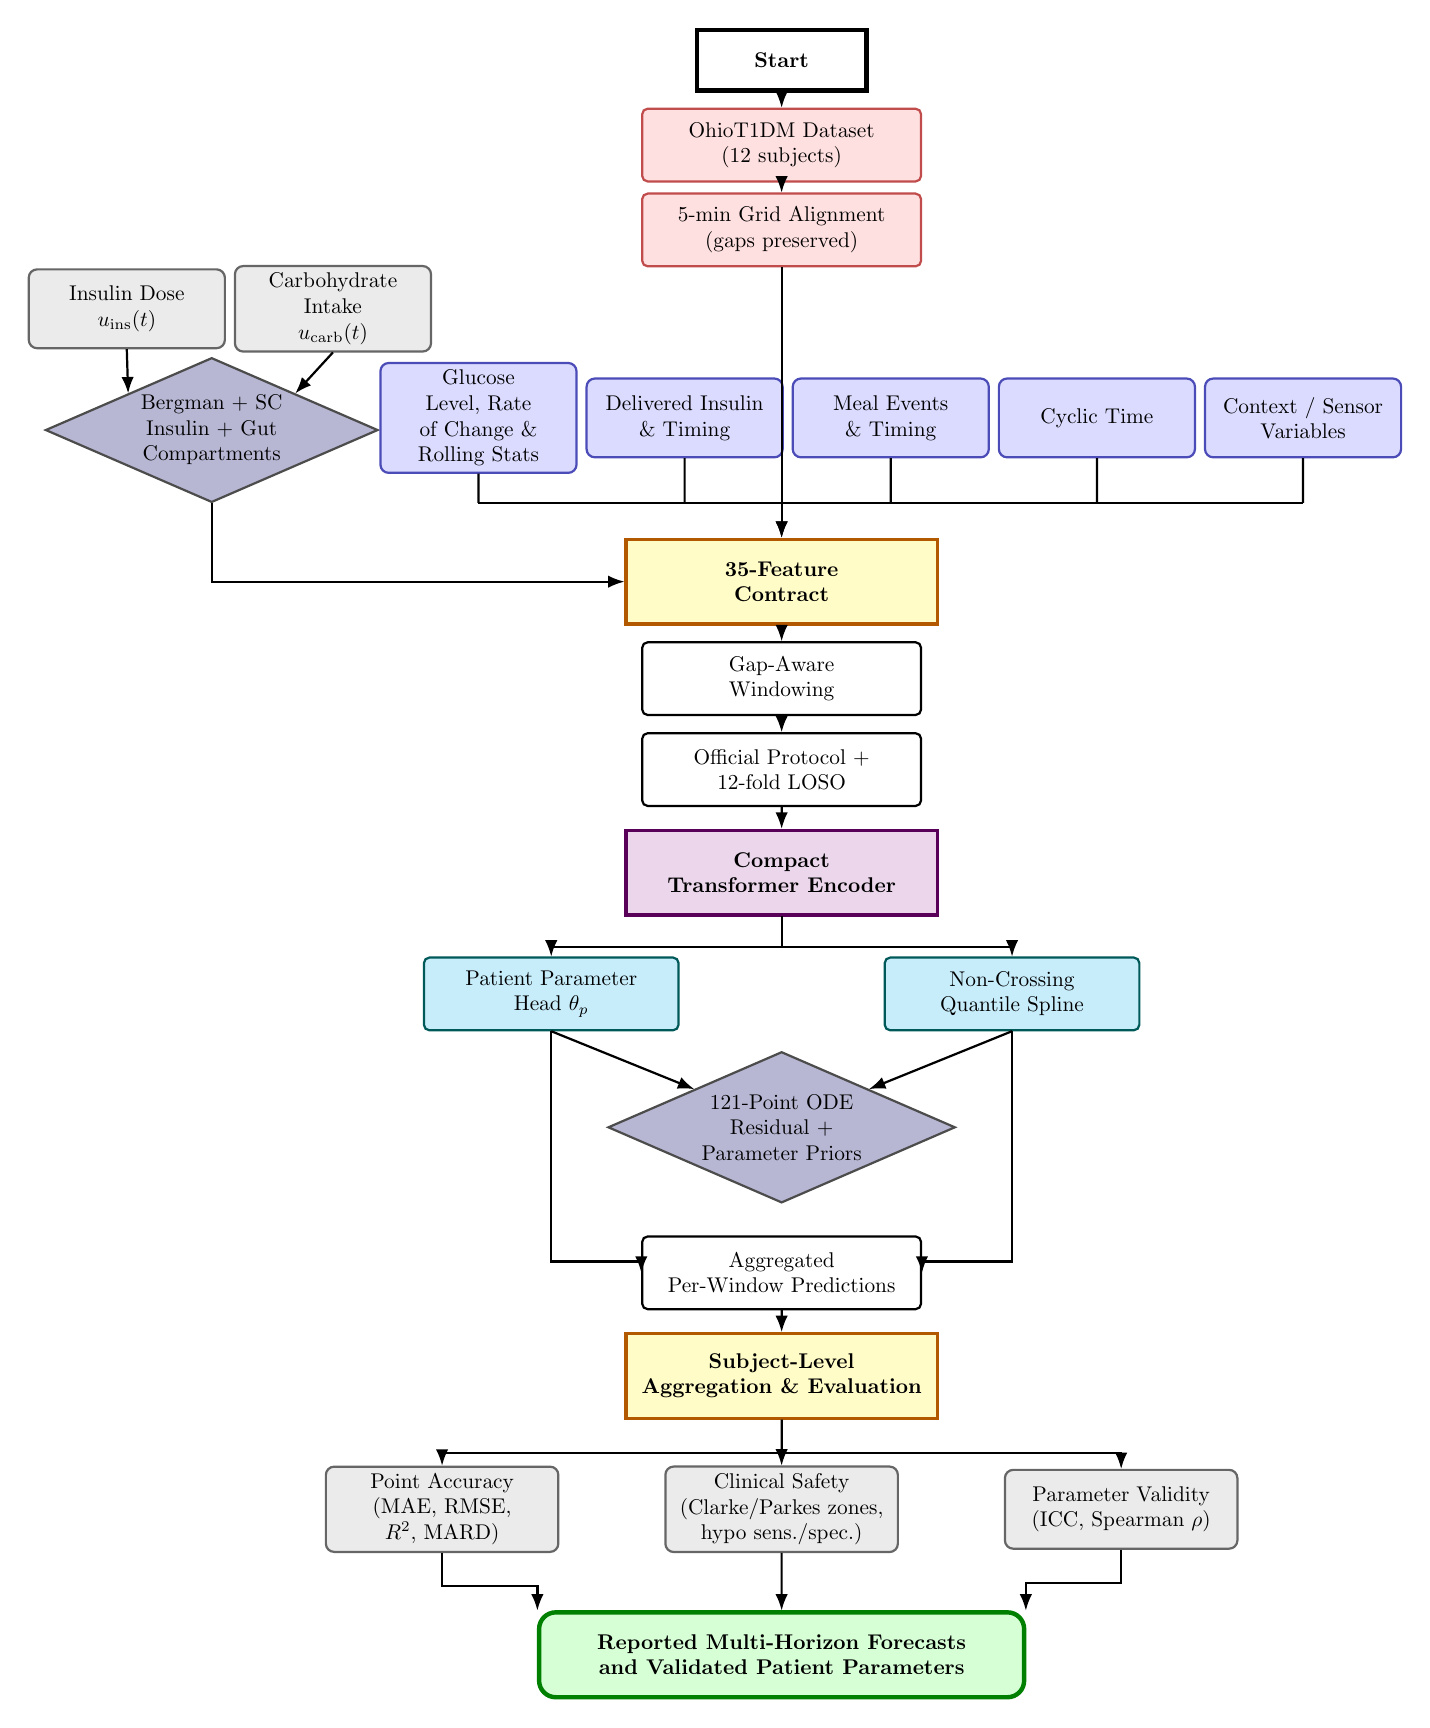
\begin{tikzpicture}[
  scale=0.77,
  transform shape,
  font=\normalsize,
  every node/.style={font=\normalsize},
  start/.style={
    rectangle, draw=black, line width=1.6pt, fill=white,
    minimum width=2.8cm, minimum height=1.0cm, align=center,
    font=\normalsize\bfseries
  },
  intake/.style={
    rectangle, rounded corners=2pt, draw=red!65!black!70, thick, fill=red!12,
    minimum width=4.6cm, minimum height=1.2cm,
    align=center, text width=4.3cm
  },
  proc/.style={
    rectangle, rounded corners=2pt, draw=black, thick, fill=white,
    minimum width=4.6cm, minimum height=1.2cm,
    align=center, text width=4.3cm
  },
  input/.style={
    rectangle, rounded corners=3pt, draw=black!60, thick, fill=black!8,
    minimum width=3.2cm, minimum height=1.3cm,
    align=center, text width=3.0cm
  },
  feat/.style={
    rectangle, rounded corners=3pt, draw=blue!60!black!70, thick, fill=blue!14,
    minimum width=3.2cm, minimum height=1.3cm,
    align=center, text width=3.0cm
  },
  hub/.style={
    chamfered rectangle,
    chamfered rectangle corners=north east and south west,
    draw=orange!70!black, very thick, fill=yellow!22,
    minimum width=5.0cm, minimum height=1.4cm,
    align=center, text width=4.7cm,
    font=\normalsize\bfseries
  },
  model/.style={
    chamfered rectangle,
    chamfered rectangle corners=north east and south west,
    draw=violet!70!black, very thick, fill=violet!16,
    minimum width=5.0cm, minimum height=1.4cm,
    align=center, text width=4.7cm,
    font=\normalsize\bfseries
  },
  head/.style={
    rectangle, rounded corners=2pt, draw=teal!70!black, thick, fill=cyan!22,
    minimum width=4.2cm, minimum height=1.2cm,
    align=center, text width=3.9cm
  },
  leaf/.style={
    rectangle, rounded corners=3pt, draw=black!60, thick, fill=black!8,
    minimum width=3.8cm, minimum height=1.3cm,
    align=center, text width=3.6cm
  },
  junction/.style={
    diamond, draw=black!70, thick, fill=blue!25!gray!45,
    aspect=2.3, align=center, inner sep=1pt,
    text width=3.0cm
  },
  final/.style={
    rectangle, rounded corners=6pt, draw=green!50!black, line width=1.6pt,
    fill=green!16,
    minimum width=8.0cm, minimum height=1.4cm,
    align=center, text width=7.6cm,
    font=\normalsize\bfseries
  },
  arr/.style={
    -{Latex[length=2.1mm]}, thick
  }
]

% Main spine
\node[start] (start) at (0,0) {Start};

\node[intake] (dataset) at (0,-1.4)
{OhioT1DM Dataset\\(12 subjects)};

\node[intake] (grid) at (0,-2.8)
{5-min Grid Alignment\\(gaps preserved)};

% Feature groups
\node[junction, text width=2.6cm] (bergman) at (-9.4,-6.1)
{Bergman + SC\\Insulin + Gut\\Compartments};

\node[feat] (fg1) at (-5.0,-5.9)
{Glucose Level, Rate\\of Change \& Rolling Stats};

\node[feat] (fg2) at (-1.6,-5.9)
{Delivered Insulin\\\& Timing};

\node[feat] (fg3) at (1.8,-5.9)
{Meal Events\\\& Timing};

\node[feat] (fg4) at (5.2,-5.9)
{Cyclic Time};

\node[feat] (fg5) at (8.6,-5.9)
{Context / Sensor\\Variables};

\node[input] (uins) at (-10.8,-4.1)
{Insulin Dose\\$u_{\text{ins}}(t)$};

\node[input] (ucarb) at (-7.4,-4.1)
{Carbohydrate Intake\\$u_{\text{carb}}(t)$};

\node[hub] (feat) at (0,-8.6)
{35-Feature\\Contract};

\node[proc] (window) at (0,-10.2)
{Gap-Aware\\Windowing};

\node[proc] (proto) at (0,-11.7)
{Official Protocol +\\12-fold LOSO};

\node[model] (xfmr) at (0,-13.4)
{Compact\\Transformer Encoder};

\node[head] (thetap) at (-3.8,-15.4)
{Patient Parameter\\Head $\theta_p$};

\node[head] (spline) at (3.8,-15.4)
{Non-Crossing\\Quantile Spline};

\node[junction] (phys) at (0,-17.6)
{121-Point ODE\\Residual +\\Parameter Priors};

\node[proc] (agg) at (0,-20.0)
{Aggregated\\Per-Window Predictions};

\node[hub] (eval) at (0,-21.7)
{Subject-Level\\Aggregation \& Evaluation};

\node[leaf] (acc) at (-5.6,-23.9)
{Point Accuracy\\(MAE, RMSE, $R^2$, MARD)};

\node[leaf] (safe) at (0,-23.9)
{Clinical Safety\\(Clarke/Parkes zones,\\hypo sens./spec.)};

\node[leaf] (valid) at (5.6,-23.9)
{Parameter Validity\\(ICC, Spearman $\rho$)};

\node[final] (outcome) at (0,-26.3)
{Reported Multi-Horizon Forecasts\\and Validated Patient Parameters};

% Mechanistic branch
\draw[arr] (uins.south) -- (bergman.north west);
\draw[arr] (ucarb.south) -- (bergman.north east);
\draw[arr] (bergman.south) |- (feat.west);

% Feature merge
\draw[thick] (fg1.south) -- (-5.0,-7.3);
\draw[thick] (fg2.south) -- (-1.6,-7.3);
\draw[thick] (fg3.south) -- (1.8,-7.3);
\draw[thick] (fg4.south) -- (5.2,-7.3);
\draw[thick] (fg5.south) -- (8.6,-7.3);
\draw[thick] (-5.0,-7.3) -- (8.6,-7.3);
\draw[arr] (0,-7.3) -- (feat.north);

% Main vertical spine
\draw[arr] (start) -- (dataset);
\draw[arr] (dataset) -- (grid);
\draw[arr] (grid.south) -- (feat.north);
\draw[arr] (feat) -- (window);
\draw[arr] (window) -- (proto);
\draw[arr] (proto) -- (xfmr);

% Transformer heads
\draw[arr] (xfmr.south) -- ++(0,-0.5) -| (thetap.north);
\draw[arr] (xfmr.south) -- ++(0,-0.5) -| (spline.north);

% Physics check
\draw[arr] (thetap.south) -- (phys.north west);
\draw[arr] (spline.south) -- (phys.north east);

% Forward path
\draw[arr] (thetap.south) -- ++(0,-3.8) -| (agg.west);
\draw[arr] (spline.south) -- ++(0,-3.8) -| (agg.east);

\draw[arr] (agg) -- (eval);

% Evaluation
\draw[arr] (eval.south) -- ++(0,-0.55) -| (acc.north);
\draw[arr] (eval) -- (safe);
\draw[arr] (eval.south) -- ++(0,-0.55) -| (valid.north);

% Final outcome
\draw[arr] (acc.south) -- ++(0,-0.55) -| (outcome.north west);
\draw[arr] (safe) -- (outcome);
\draw[arr] (valid.south) -- ++(0,-0.55) -| (outcome.north east);

\end{tikzpicture}

\caption{\small\textit{Audited forecasting pipeline of the hybrid physics-guided model. OhioT1DM glucose and related patient data are aligned to five-minute intervals and processed through two parallel paths: a deep-learning model and a physiological model. The deep-learning model predicts future glucose levels and estimates patient-specific parameters, while the physiological model represents insulin and glucose dynamics. Physiological information is used both as an input to the model and as a training constraint to improve prediction consistency.
}}
\label{fig:pipeline}
\end{figure*}

\subsection{Mechanistic Patient Model}

The physiological core extends the Bergman minimal model and its insulin-sensitivity index~\cite{ref1,ref32}, as given in Eqs.~\eqref{eq:2}--\eqref{eq:4}:
\begin{align}
\dot{G} &= -(p_1 + X)\,G + p_1 G_b + \frac{R_a(t)}{V_G}, \label{eq:2}\\
\dot{X} &= -p_2 X + p_3 (I - I_b), \label{eq:3}\\
\dot{I} &= -nI + \frac{1000}{V_I}\cdot\frac{S_2}{t_{\max,I}}. \label{eq:4}
\end{align}

Here $G$ is glucose, $I$ plasma insulin, $X$ remote insulin action, and subscript $b$ denotes basal state. All rates are per minute. Basal subtraction in (\ref{eq:3}) is essential: at $I = I_b$, $X^* = 0$ and $G = G_b$ is an equilibrium. Driving the equation with total insulin instead would create a spurious downward glucose attractor.

The patient-specific insulin sensitivity is the steady-state gain, as given in Eq.~\eqref{eq:5}:
\begin{equation}
S_I = \frac{p_3}{p_2}, \qquad X_{ss} = S_I (I - I_b),
\label{eq:5}
\end{equation}
with units mL\,$\mu$U$^{-1}$min$^{-1}$. Parameters are mapped by sigmoid functions into physiologically sourced intervals informed by minimal-model studies in insulin-dependent diabetes~\cite{ref33} and regularized toward population anchors. Consequently, plausible range alone is not evidence of identifiability; external and stability checks are required.

Subcutaneous insulin absorption follows a two-compartment model~\cite{ref34}, as given in Eqs.~\eqref{eq:6}--\eqref{eq:8}:
\begin{align}
\dot{S}_1 &= u_{\text{ins}}(t) - \frac{S_1}{t_{\max,I}}, \label{eq:6}\\
\dot{S}_2 &= \frac{S_1}{t_{\max,I}} - \frac{S_2}{t_{\max,I}}. \label{eq:7}
\end{align}

For an impulse dose $D$, insulin on board is
\begin{equation}
S_1 + S_2 = D\,e^{-t/t_{\max,I}}\left(1 + \frac{t}{t_{\max,I}}\right),
\label{eq:8}
\end{equation}
which starts at $D$ and decreases monotonically. Carbohydrate absorption follows compartmental meal models used in T1D simulation~[\hyperref[ref35label]{44}-\hyperref[ref37label]{46}] and is represented by stomach and gut states, as given in Eqs.~\eqref{eq:9}--\eqref{eq:11}:
\begin{align}
\dot{Q}_{\text{sto}} &= -k_{\text{gri}} Q_{\text{sto}} + u_{\text{carb}}(t), \label{eq:9}\\
\dot{Q}_{\text{gut}} &= k_{\text{gri}} Q_{\text{sto}} - k_{\text{abs}} Q_{\text{gut}}, \label{eq:10}\\
R_a(t) &= f\, k_{\text{abs}} Q_{\text{gut}}(t), \label{eq:11}
\end{align}
so carbohydrate on board is $Q_{\text{sto}} + Q_{\text{gut}}$ and absorbed mass is conserved. For implementation, the non-glucose compartments are collected, as given in Eq.~\eqref{eq:12}:
\begin{equation}
\mathbf{z} = {[S_1, S_2, I, Q_{\text{sto}}, Q_{\text{gut}}, X]}^{\mathsf T}, \quad \mathbf{u} = {[u_{\text{ins}}, u_{\text{carb}}, I_b]}^{\mathsf T}.
\label{eq:12}
\end{equation}

With parameters held constant over one grid interval, $\dot{\mathbf{z}} = A\mathbf{z} + B\mathbf{u}$ has the exact zero-order-hold update (a standard control-theory discretization technique, not attributed to a specific glucose-modeling source), as given in Eq.~\eqref{eq:13}:
\begin{equation}
\mathbf{z}_{k+1} = A_d \mathbf{z}_k + B_d \mathbf{u}_k, \qquad
\begin{bmatrix} A_d & B_d \\ 0 & I \end{bmatrix} = \exp\!\left(\Delta \begin{bmatrix} A & B \\ 0 & 0 \end{bmatrix}\right).
\label{eq:13}
\end{equation}

This matrix-exponential formulation preserves the affine basal term through the explicit $I_b$ input and avoids the accumulated integration error of a coarse explicit solver.

\subsection{Feature Contract and Forecasting Network}

Each timestep contains 35 named features in six groups: glucose level, multiscale rates of change and rolling statistics; delivered insulin and timing; meals and timing; mechanistic states (IOB, COB, plasma insulin, remote action, and glucose appearance); cyclic time; and context/sensor variables. A two-hour window $X \in \mathbb{R}^{24 \times 35}$ is standardized using training-only statistics.

The forecasting network is deliberately small (approximately 79,000 parameters) because the effective sample size is limited. A linear projection and positional encoding feed a Transformer encoder~\cite{ref38}. Attention pooling, Eq.~\eqref{eq:14}, gives
\begin{equation}
z = \sum_{t=1}^{24} \alpha_t h_t, \qquad \alpha_t = \frac{\exp(w^\top h_t)}{\sum_j \exp(w^\top h_j)},
\label{eq:14}
\end{equation}
avoiding the equal weighting of old and recent measurements induced by mean pooling.

One head estimates the ten-component subject parameter vector $\theta_p$. A second predicts a cubic B-spline trajectory, as given in Eq.~\eqref{eq:15}:
\begin{equation}
G_\theta(t) = G_0 + \sum_{k=1}^{K} c_k \big(B_k(t) - B_k(0)\big),
\label{eq:15}
\end{equation}
which anchors every trajectory at the last observed glucose $G_0$. Median knot values are unconstrained, whereas lower and upper quantiles are generated by positive softplus offsets in glucose units; quantiles therefore cannot cross. A learned trust gate $g = \sigma(\gamma)$ controls the contribution of the mechanistic prior, with $g \approx 0.10$ at initialization. Predictions at all four horizons are evaluated from the spline.

\subsection{Training Objective}

The data objective combines Huber's robust loss~\cite{ref39} for the median with the pinball loss used in quantile regression~\cite{ref40} for lower and upper quantiles, as given in Eq.~\eqref{eq:16}:
\begin{equation}
\mathcal{L}_{\text{data}} = \mathcal{L}_{\text{Huber}}(y, \hat{y}_{0.5}) + \sum_{q \in \{0.1, 0.9\}} \rho_q(y - \hat{y}_q),
\label{eq:16}
\end{equation}
where $\rho_q(u) = u(q - \mathbb{1}_{u<0})$. Physics residuals are evaluated at 121 collocation points over the two-hour forecast and normalized by physiological scales, following the residual-minimization principle of PINNs~\cite{ref8}. The full objective is given in Eq.~\eqref{eq:17}:
\begin{equation}
\mathcal{L} = \mathcal{L}_{\text{data}} + \lambda_{\text{phys}} \mathcal{L}_{\text{phys}} + \lambda_{\text{prior}} \mathcal{L}_{\text{prior}} + \lambda_{\text{tc}} \mathcal{L}_{\text{temporal}}.
\label{eq:17}
\end{equation}

Closed-form state updates replace a memory-intensive differentiable ODE solver. Adaptive loss weighting was motivated by work on gradient imbalance and uncertainty-based multi-objective learning~[\hyperref[ref41label]{50}-\hyperref[ref42label]{51}]. The selected A7 configuration applies physics from epoch one; a data-first curriculum was rejected because validation optima repeatedly occurred before the curriculum became selectable.

\subsection{Evaluation and Statistical Analysis}

The official temporal protocol uses each subject's earlier data for training. LOSO trains on 11 subjects and evaluates the held-out subject on the identical test windows. Metrics are computed per subject and summarized as mean $\pm$ SD\@. Persistence predicts $\hat{G}(t+h) = G(t)$. Skill is $1 - \text{RMSE}_{\text{model}}/\text{RMSE}_{\text{persistence}}$, computed from the cohort-mean RMSEs.

Clinical evaluation includes Clarke and Parkes zones~[\hyperref[ref43label]{52}-\hyperref[ref45label]{54}], consensus CGM ranges~\cite{ref52}, coefficient-of-variation ratio, and Kovatchev low/high blood-glucose risk indices~[\hyperref[ref46label]{56}-\hyperref[ref47label]{57}], together with hypoglycemia sensitivity, specificity, precision, and quantile calibration. Paired model comparisons use the Wilcoxon signed-rank test~\cite{ref48} across 12 subjects with Holm multiplicity correction~\cite{ref49}; bootstrap intervals resample subjects, never overlapping windows. Test--retest reliability of $S_I$ is measured with one-way ICC(1)~\cite{ref50}, and concurrent validity uses Spearman rank correlation~\cite{ref51}.

\subsection{Preregistered Outcomes and Falsification Criteria}

The primary outcome is 30-minute MAE under the official protocol for the physiology-focused branch. Secondary outcomes include all horizons under both protocols, persistence skill, Clarke, Parkes, and PRED-EGA distributions, the ablation matrix, quantile calibration, and the three $S_I$ validation checks. Table~\ref{tab:falsification} records the criteria that were fixed in advance; unmet criteria are reported as failures rather than redefined after inspection.

No asymmetric hypoglycemia/hyperglycemia point-loss term is permitted, because such a term would directly optimize the safety table later used as evidence. The test set is evaluated only after model selection, and the official protocol is never described as subject-disjoint generalization.

\subsection{Reproducibility, Hardware, and Latency}

Models were implemented in PyTorch 2.10 (CUDA 12.8) and trained with AdamW (learning rate $5 \times 10^{-4}$, weight decay 0.03, batch size 256, gradient clipping at $L_2$ norm 1.0) for at most 70 epochs, with early stopping after 12 epochs without improvement in validation MAE averaged across horizons. The hyperparameter search covered encoder depth $\in \{2, 4\}$, $d_{\text{model}} \in \{64, 128\}$, attention heads $\in \{4, 8\}$, $d_{\text{ff}} \in \{128, 512\}$, dropout $\in \{0.1, 0.2\}$, pooling (attention, mean, or last), and physics-loss weighting (fixed $\lambda_{\text{phys}} \in [0.01, 1.0]$ vs.\ Kendall homoscedastic uncertainty weighting).

Experiments ran on a single Linux machine with an NVIDIA GeForce RTX 2050 Laptop GPU (4~GB) and an Intel Core CPU. Training took about 23~s per epoch (about 4.5~min per run). Inference latency for one window (batch size 1, 100 forward passes) was $15.25 \pm 4.07$~ms on GPU (median 13.21~ms, 95th percentile 25.07~ms) and $6.33 \pm 0.18$~ms on CPU (median 6.31~ms), well within the 5-minute CGM sampling interval. Code, data-processing pipelines, and configurations are available at \url{https://github.com/sammyyakk/digital-twin}.

\subsection{Feature Attribution Method}

Integrated gradients (IG)~\cite{ref54} uses the standardized training mean as its zero baseline, as given in Eq.~\eqref{eq:18}:
\begin{equation}
\text{IG}_i(x) = (x_i - x_i') \int_0^1 \frac{\partial f(x' + \alpha(x - x'))}{\partial x_i}\, d\alpha.
\label{eq:18}
\end{equation}

Because IG shows an unresolved completeness violation, every interpretation is cross-checked with model-agnostic permutation importance, following the perturbation principle popularized for random forests~\cite{ref55}.

\begin{table*}[t]
\centering
\caption{Preregistered success and falsification criteria}
\label{tab:falsification}
\footnotesize
\begin{tabular}{>{\raggedright\arraybackslash}p{2.6cm}>{\raggedright\arraybackslash}p{5.6cm}>{\raggedright\arraybackslash}p{5.8cm}>{\raggedright\arraybackslash}p{2.4cm}}
\toprule
Claim & Criterion fixed before test evaluation & Interpretation & Ref. \\
\midrule
Beats persistence & 30-minute MAE below persistence in at least 10 of 12 subjects & Requires broadly distributed improvement, not a pooled gain driven by a few subjects. & [\hyperref[ref30label]{38}-\hyperref[ref31label]{39}],~\cite{ref57} \\
Field-competitive point accuracy & 30-minute MAE $\leq$ 13.5 mg/dL & A field-relative target, explicitly not a clinical acceptability threshold. &~\cite{ref31},~[\hyperref[ref43label]{52}-\hyperref[ref44label]{53}],~\cite{ref64} \\
Physics improves accuracy & Physics arm beats A0 at 30 minutes and survives paired Wilcoxon testing with Holm correction & If unmet, physics is not credited with point-accuracy improvement. & [\hyperref[ref48label]{58}-\hyperref[ref49label]{59}] \\
$S_I$ is subject-specific & Between-subject CV $>$ 10\% & Rejects a parameter head collapsed to one population value. &~\cite{ref1,ref32} \\
$S_I$ is stable & ICC(1) $>$ 0.5 on disjoint within-subject blocks & Rejects a window-level nuisance variable that merely absorbs prediction error. &~\cite{ref50,ref76} \\
$S_I$ is externally consistent & Spearman $\rho < 0$ versus total daily dose, with a subject-bootstrap 95\% CI excluding zero & Evaluated separately under personalized and LOSO protocols. &~\cite{ref51},~[\hyperref[ref77label]{66}-\hyperref[ref78label]{67}] \\
\bottomrule
\end{tabular}
\end{table*}


%=================================================================
\section{Results}

\subsection{Baseline Validation and Data Accounting}

Persistence RMSE on the 2018 cohort is $22.52 \pm 2.56$~mg/dL at 30 minutes and $36.19 \pm 3.26$~mg/dL at 60 minutes, within $0.02$~mg/dL of both independently published no-change baselines at 30 minutes and within $0.41$~mg/dL of the published 60-minute value[\hyperref[ref56label]{36}-\hyperref[ref57label]{37}]. This close agreement validates the complete evaluation pipeline, including data parsing, five-minute grid alignment, horizon construction, persistence-target generation, RMSE computation, and subject-level aggregation (Table~\ref{tab:windows}). The retained-window accounting further confirms that the reported metrics are computed on the intended 26,498 common test windows. 

\begin{table}[t]
\centering
\caption{Window accounting after integrity filtering. All 12 subjects (2018 and 2020 cohorts); counts are totals across subjects, and the 26,498 test windows are shared by both evaluation protocols.}
\label{tab:windows}
\footnotesize
\begin{tabular}{lr}
\toprule
Quantity & Value \\
\midrule
Subjects / CGM observations & 12 / 166,443 \\
Candidate windows & 187,780 \\
Retained windows & 141,100 (75.1\%) \\
Incomplete input span & 36,395 \\
Missing real target & 10,285 \\
Common test windows & 26,498 \\
Effective independent windows & $\approx 2{,}800$ \\
\bottomrule
\end{tabular}
\end{table}

\subsection{Official-Protocol Forecast Accuracy}

Table~\ref{tab:official} and Fig.~\ref{fig:summary} show that the model improves on persistence at every horizon. All 12 subjects improve at 30 minutes; subject-level MAE skill ranges from 12.2\% to 31.6\%. The decline in $R^2$ with horizon is expected because future meals, boluses, and activity are absent from the input.

\pgfplotstableread[col sep=comma]{data/mae_by_horizon.csv}\maetable
\pgfplotstableread[col sep=comma]{data/rmse_by_horizon.csv}\rmsetable
\pgfplotstablegetelem{0}{mean}\of\maetable \global\let\maePersA=\pgfplotsretval
\pgfplotstablegetelem{1}{mean}\of\maetable \global\let\maePersB=\pgfplotsretval
\pgfplotstablegetelem{2}{mean}\of\maetable \global\let\maePersC=\pgfplotsretval
\pgfplotstablegetelem{3}{mean}\of\maetable \global\let\maePersD=\pgfplotsretval
\pgfplotstablegetelem{4}{mean}\of\maetable \global\let\maeModA=\pgfplotsretval
\pgfplotstablegetelem{5}{mean}\of\maetable \global\let\maeModB=\pgfplotsretval
\pgfplotstablegetelem{6}{mean}\of\maetable \global\let\maeModC=\pgfplotsretval
\pgfplotstablegetelem{7}{mean}\of\maetable \global\let\maeModD=\pgfplotsretval
\pgfplotstablegetelem{0}{mean}\of\rmsetable \global\let\rmsePersA=\pgfplotsretval
\pgfplotstablegetelem{1}{mean}\of\rmsetable \global\let\rmsePersB=\pgfplotsretval
\pgfplotstablegetelem{2}{mean}\of\rmsetable \global\let\rmsePersC=\pgfplotsretval
\pgfplotstablegetelem{3}{mean}\of\rmsetable \global\let\rmsePersD=\pgfplotsretval
\pgfplotstablegetelem{4}{mean}\of\rmsetable \global\let\rmseModA=\pgfplotsretval
\pgfplotstablegetelem{5}{mean}\of\rmsetable \global\let\rmseModB=\pgfplotsretval
\pgfplotstablegetelem{6}{mean}\of\rmsetable \global\let\rmseModC=\pgfplotsretval
\pgfplotstablegetelem{7}{mean}\of\rmsetable \global\let\rmseModD=\pgfplotsretval
\pgfmathsetmacro{\skillA}{100*(1-\rmseModA/\rmsePersA)}
\pgfmathsetmacro{\skillB}{100*(1-\rmseModB/\rmsePersB)}
\pgfmathsetmacro{\skillC}{100*(1-\rmseModC/\rmsePersC)}
\pgfmathsetmacro{\skillD}{100*(1-\rmseModD/\rmsePersD)}


% Core packages


% Paragraphs
\begin{figure*}[t]
\centering

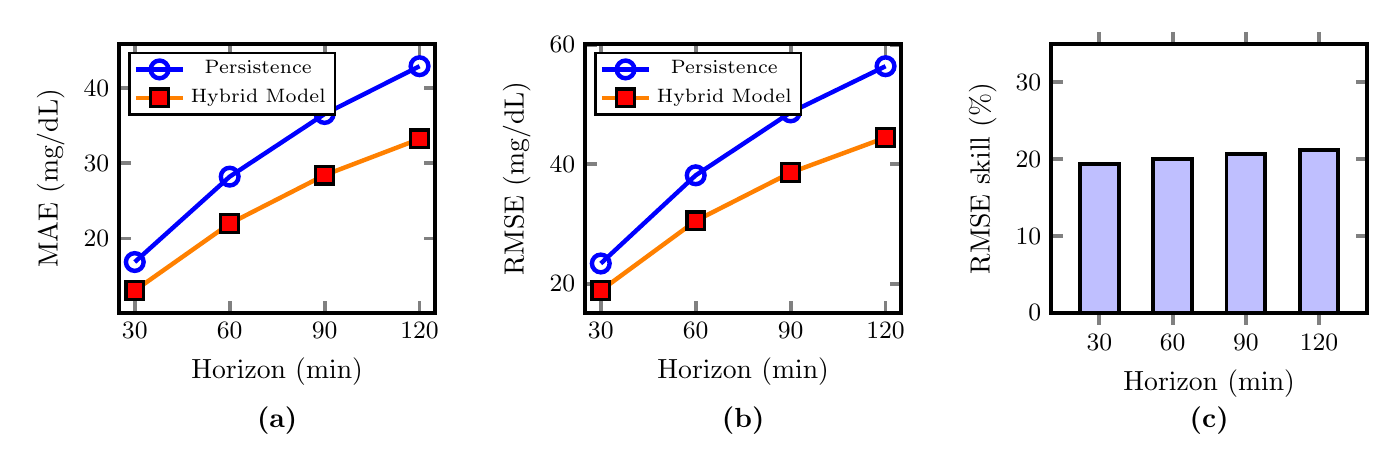
\begin{tikzpicture}
\begin{groupplot}[
  group style={group size=3 by 1, horizontal sep=1.9cm},
  width=5.6cm, height=5.0cm,
  xlabel={Horizon (min)},
  xtick={30,60,90,120},
  axis line style={line width=1.4pt},
  tick style={line width=1.4pt},
  label style={font=\normalsize},
  tick label style={font=\small},
  title style={font=\normalsize\bfseries, yshift=-0.7em},
]

% ---------- (a) MAE ----------
\nextgroupplot[
  ylabel={MAE (mg/dL)},
  xmin=25, xmax=125,
  legend pos=north west,
  legend style={
    font=\scriptsize,
    line width=0.8pt,
    draw=black,
    inner xsep=1.5pt,
    inner ysep=0.8pt
},
  title={(a)},
  title style={at={(0.5,-0.30)}, anchor=north},
]
\addplot[
  color=blue, line width=1.6pt, mark=o, mark options={scale=1.6, line width=1.6pt, fill=none},
] coordinates {
  (30,16.87) (60,28.22) (90,36.55) (120,42.90)
};
\addlegendentry{Persistence}

\addplot[
  color=orange, line width=1.6pt, mark=square*,
  mark options={scale=1.6, line width=1.2pt, fill=red, draw=black},
] coordinates {
  (30,13.08) (60,21.98) (90,28.42) (120,33.23)
};
\addlegendentry{Hybrid Model}

% ---------- (b) RMSE ----------
\nextgroupplot[
  ylabel={RMSE (mg/dL)},
  xmin=25, xmax=125,
  legend pos=north west,
  legend style={
    font=\scriptsize,
    line width=0.8pt,
    draw=black,
    inner xsep=1.5pt,
    inner ysep=0.8pt
},
  title={(b)},
  title style={at={(0.5,-0.30)}, anchor=north},
]
\addplot[
  color=blue, line width=1.6pt, mark=o, mark options={scale=1.6, line width=1.6pt, fill=none},
] coordinates {
  (30,23.37) (60,38.15) (90,48.69) (120,56.43)
};
\addlegendentry{Persistence}

\addplot[
  color=orange, line width=1.6pt, mark=square*,
  mark options={scale=1.6, line width=1.2pt, fill=red, draw=black},
] coordinates {
  (30,18.84) (60,30.52) (90,38.60) (120,44.46)
};
\addlegendentry{Hybrid Model}

% ---------- (c) RMSE skill ----------
\nextgroupplot[
  ylabel={RMSE skill (\%)},
  ybar,
  bar width=14pt,
  ymin=0, ymax=35,
  xtick=data,
  symbolic x coords={30,60,90,120},
  enlarge x limits=0.22,
  title={(c)},
  title style={at={(0.5,-0.30)}, anchor=north},
]
\addplot[
  fill=blue!25, draw=black, line width=1.4pt,
] coordinates {
  (30,19.4) (60,20.0) (90,20.7) (120,21.2)
};
\end{groupplot}
\end{tikzpicture}

\caption{\small\textit{Official-protocol accuracy summary at 30/60/90/120 minutes. (a) and (b): MAE and RMSE for persistence versus the hybrid model both rise with horizon, but the gap between the two curves widens rather than closes, showing the model's advantage over naive persistence is not a short-horizon artifact. (c): the resulting RMSE skill stays essentially flat at 19--21\% across all four horizons.}}
\label{fig:summary}
\end{figure*}





\begin{table*}[t]
\centering
\caption{Official personalized protocol, all 12 subjects, final model (median of the quantile-head run): mean $\pm$ SD across subjects (mg/dL unless noted). These values come from the final-model run, which was trained separately from ablation arm A7 in Tables~\ref{tab:baselines_identical} and~\ref{tab:ablation}; this explains the small differences (e.g., 30-min MAE 13.08 here vs.\ 13.25 there).}
\label{tab:official}
\footnotesize
\begin{tabular}{lrrrrrrr}
\toprule
Horizon & Persistence MAE & Model MAE & Persistence RMSE & Model RMSE & RMSE skill & $R^2$ & MARD \\
\midrule
30 min & 16.87 $\pm$ 1.92 & \textbf{13.08 $\pm$ 1.73} & 23.37 & \textbf{18.84 $\pm$ 2.58} & 19.4\% & 0.885 & 8.79\% \\
60 min & 28.22 $\pm$ 3.24 & \textbf{21.98 $\pm$ 2.96} & 38.15 & \textbf{30.52 $\pm$ 3.98} & 20.0\% & 0.700 & 14.76\% \\
90 min & 36.55 $\pm$ 4.00 & \textbf{28.42 $\pm$ 3.89} & 48.69 & \textbf{38.60 $\pm$ 5.05} & 20.7\% & 0.523 & 19.14\% \\
120 min & 42.90 $\pm$ 4.46 & \textbf{33.23 $\pm$ 4.45} & 56.43 & \textbf{44.46 $\pm$ 5.62} & 21.2\% & 0.368 & 22.37\% \\
\bottomrule
\end{tabular}
\end{table*}

\subsection{Comprehensive Baseline Comparison on Identical Windows}
\label{sec:baselines_identical}

Table~\ref{tab:baselines_identical} compares nine models on the same 26,498 test windows from all 12 subjects under the official protocol:
\begin{enumerate}
    \item \textbf{Persistence:} zero-order hold, $\hat{G}_{t+h} = G_t$.
    \item \textbf{Bergman ODE, population parameters:} forward integration from the basal steady state with literature parameters~\cite{ref1,ref32}, without neural correction.
    \item \textbf{Bergman ODE, per-subject fit:} parameters fitted per subject by nonlinear least squares/MAP on historical calibration intervals.
    \item \textbf{AR(6):} linear autoregression on the last six CGM values (30-min lookback).
    \item \textbf{ARX(6):} AR(6) with added insulin and carbohydrate inputs.
    \item \textbf{LSTM:} recurrent model on the 26 non-mechanistic features.
    \item \textbf{Transformer, $A0_{\text{no-mech}}$:} the hybrid model's backbone trained on the same 26 features.
    \item \textbf{Transformer, A0:} the same backbone with all 35 features, including mechanistic insulin- and carbohydrate-on-board.
    \item \textbf{Hybrid physics-guided, A7:} A0 plus the Bergman prior, learned residual correction, and parameter head.
\end{enumerate}

Mechanistic models alone performed worst: with population parameters the ODE drifted to a 30-min MAE of 29.70~mg/dL (54.18~mg/dL at 120~min), and per-subject fitting improved this only to 25.80~mg/dL (48.43~mg/dL at 120~min). Linear models were competitive: AR(6) beat persistence by 2.48~mg/dL at 30~min, and adding insulin and meal inputs (ARX) lowered MAE to 13.97~mg/dL. Adding mechanistic features to the Transformer reduced 30-min MAE by 1.45~mg/dL (14.96 to 13.51~mg/dL), and A7 had the lowest MAE at every horizon in this comparison (13.25~mg/dL at 30~min).

\begin{table*}[t]
\centering
\caption{Comprehensive baseline comparison across 12 subjects evaluated on identical test windows ($n=26{,}498$). Metrics reported as mean $\pm$ SD across subjects (mg/dL). The A7 row is the single-seed ablation run (as in Table~\ref{tab:ablation}), not the final model in Table~\ref{tab:official}.}
\label{tab:baselines_identical}
\footnotesize
\setlength{\tabcolsep}{2.3pt}
\begin{tabular}{lrrrrrrrr}
\toprule
& \multicolumn{2}{c}{30 min} & \multicolumn{2}{c}{60 min} & \multicolumn{2}{c}{90 min} & \multicolumn{2}{c}{120 min} \\
\cmidrule(lr){2-3} \cmidrule(lr){4-5} \cmidrule(lr){6-7} \cmidrule(lr){8-9}
Model & MAE & RMSE & MAE & RMSE & MAE & RMSE & MAE & RMSE \\
\midrule
Persistence & 16.87$\,\pm\,$1.92 & 23.37$\,\pm\,$2.85 & 28.22$\,\pm\,$3.24 & 38.15$\,\pm\,$4.58 & 36.55$\,\pm\,$4.00 & 48.69$\,\pm\,$5.58 & 42.90$\,\pm\,$4.46 & 56.43$\,\pm\,$6.21 \\
Bergman ODE (population) & 29.70$\,\pm\,$9.67 & 39.67$\,\pm\,$12.67 & 43.71$\,\pm\,$12.84 & 57.08$\,\pm\,$16.10 & 50.72$\,\pm\,$13.66 & 65.26$\,\pm\,$16.79 & 54.18$\,\pm\,$13.78 & 69.20$\,\pm\,$16.77 \\
Bergman ODE (per-subject NLS) & 25.80$\,\pm\,$8.36 & 34.72$\,\pm\,$10.45 & 38.09$\,\pm\,$9.56 & 50.41$\,\pm\,$11.78 & 44.70$\,\pm\,$8.99 & 58.47$\,\pm\,$11.01 & 48.43$\,\pm\,$8.35 & 63.03$\,\pm\,$10.29 \\
AR(6) & 14.39$\,\pm\,$1.52 & 20.11$\,\pm\,$2.65 & 25.52$\,\pm\,$2.90 & 33.88$\,\pm\,$3.90 & 33.18$\,\pm\,$3.66 & 42.92$\,\pm\,$4.62 & 38.30$\,\pm\,$3.90 & 48.64$\,\pm\,$4.92 \\
ARX(6) & 13.97$\,\pm\,$1.51 & 19.61$\,\pm\,$2.76 & 24.48$\,\pm\,$2.86 & 32.67$\,\pm\,$3.98 & 32.24$\,\pm\,$3.47 & 41.82$\,\pm\,$4.47 & 37.68$\,\pm\,$3.69 & 48.00$\,\pm\,$4.77 \\
LSTM (non-mechanistic) & 15.41$\,\pm\,$2.16 & 21.46$\,\pm\,$2.83 & 26.08$\,\pm\,$3.87 & 35.24$\,\pm\,$4.56 & 33.59$\,\pm\,$4.77 & 44.97$\,\pm\,$5.76 & 38.81$\,\pm\,$5.30 & 51.54$\,\pm\,$6.63 \\
Transformer ($A0_{\text{no-mech}}$) & 14.96$\,\pm\,$1.82 & 21.08$\,\pm\,$2.55 & 26.06$\,\pm\,$3.15 & 35.56$\,\pm\,$4.15 & 34.46$\,\pm\,$3.81 & 46.08$\,\pm\,$5.11 & 40.06$\,\pm\,$4.09 & 53.03$\,\pm\,$5.63 \\
Transformer (all features, A0) & 13.51$\,\pm\,$1.63 & 19.38$\,\pm\,$2.41 & 22.82$\,\pm\,$2.88 & 31.61$\,\pm\,$3.71 & 29.74$\,\pm\,$3.74 & 40.32$\,\pm\,$4.71 & 34.93$\,\pm\,$4.20 & 46.70$\,\pm\,$5.24 \\
\textbf{Hybrid physics-guided (A7)} & \textbf{13.25$\,\pm\,$1.69} & \textbf{19.06$\,\pm\,$2.51} & \textbf{22.29$\,\pm\,$2.93} & \textbf{30.89$\,\pm\,$3.89} & \textbf{28.77$\,\pm\,$3.75} & \textbf{39.04$\,\pm\,$4.83} & \textbf{33.38$\,\pm\,$4.21} & \textbf{44.78$\,\pm\,$5.46} \\
\bottomrule
\end{tabular}
\end{table*}

\subsection{Cross-Subject Generalization}

At 30 minutes, LOSO remains better than persistence in all 12 subjects by MAE (10 of 12 by RMSE), but is consistently worse than the personalized protocol. As Fig.~\ref{fig:matched_protocol_comparison} shows, the personalization gap grows with horizon, consistent with increasing dependence on individual insulin kinetics and routine.

\pgfplotstableread[col sep=comma]{data/loso_leaderboard_mae.csv}\losotable
\pgfplotstablegetelem{0}{mean}\of\maetable \global\let\persA=\pgfplotsretval
\pgfplotstablegetelem{1}{mean}\of\maetable \global\let\persB=\pgfplotsretval
\pgfplotstablegetelem{2}{mean}\of\maetable \global\let\persC=\pgfplotsretval
\pgfplotstablegetelem{3}{mean}\of\maetable \global\let\persD=\pgfplotsretval
\pgfplotstablegetelem{4}{mean}\of\maetable \global\let\persoA=\pgfplotsretval
\pgfplotstablegetelem{5}{mean}\of\maetable \global\let\persoB=\pgfplotsretval
\pgfplotstablegetelem{6}{mean}\of\maetable \global\let\persoC=\pgfplotsretval
\pgfplotstablegetelem{7}{mean}\of\maetable \global\let\persoD=\pgfplotsretval
\pgfplotstablegetelem{4}{mae_mean}\of\losotable \global\let\losoA=\pgfplotsretval
\pgfplotstablegetelem{5}{mae_mean}\of\losotable \global\let\losoB=\pgfplotsretval
\pgfplotstablegetelem{6}{mae_mean}\of\losotable \global\let\losoC=\pgfplotsretval
\pgfplotstablegetelem{7}{mae_mean}\of\losotable \global\let\losoD=\pgfplotsretval

\begin{figure}[t]
\centering

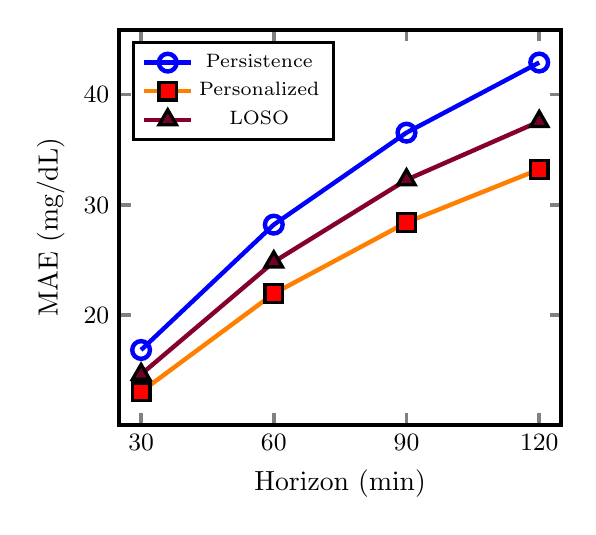
\begin{tikzpicture}
\begin{axis}[
  width= 7.2cm, height=6.6 cm,
  xlabel={Horizon (min)},
  ylabel={MAE (mg/dL)},
  xtick={30,60,90,120},
  xmin=25, xmax=125,
  axis line style={line width=1.4pt},
  tick style={line width=1.4pt},
  label style={font=\normalsize},
  tick label style={font=\small},
  legend pos=north west,
  legend style={font=\scriptsize, line width=1pt, draw=black},
]

\addplot[
  color=blue, line width=1.6pt, mark=o, mark options={scale=1.6, line width=1.6pt, fill=none},
] coordinates {
  (30,16.87) (60,28.22) (90,36.55) (120,42.90)
};
\addlegendentry{Persistence}

\addplot[
  color=orange, line width=1.6pt, mark=square*,
  mark options={scale=1.6, line width=1.2pt, fill=red, draw=black},
] coordinates {
  (30,13.08) (60,21.98) (90,28.42) (120,33.23)
};
\addlegendentry{Personalized}

\addplot[
  color=purple!70!black, line width=1.6pt, mark=triangle*,
  mark options={scale=1.8, line width=1.2pt, fill=purple!60!black, draw=black},
] coordinates {
  (30,14.66) (60,24.85) (90,32.28) (120,37.56)
};
\addlegendentry{LOSO}

\end{axis}
\end{tikzpicture}

\caption{\small\textit{Matched-protocol comparison across 30, 60, 90, and 120-minute horizons. Persistence, personalized, and LOSO models are evaluated on identical windows. LOSO keeps a roughly constant MAE advantage of about 12\% over persistence at every horizon, while its gap to the personalized model widens from 1.6 to 4.3~mg/dL, indicating a greater benefit from within-subject history for extended forecasting.}}
\label{fig:matched_protocol_comparison}
\end{figure}


\subsection{Physics Ablations}
In the pre-specified single-seed ablation, no physics configuration significantly outperformed the no-physics A0 baseline after Holm correction (Table~\ref{tab:ablation}; Fig.~\ref{fig:ablationfig}). A7 was nominally best and improved 9 of 12 subjects, but its corrected $p = 0.105$, so the pre-specified criterion was not met. A post hoc 5-seed replication of A0 and A7, not part of the pre-specified plan (Section~\ref{sec:multiseed_replication}) found that, on seed-averaged per-subject errors, A7 has lower MAE at every horizon, by 0.51~mg/dL at 30~min and 2.38~mg/dL at 120~min (Holm $p = 0.002$ at each horizon). Per-patient parameters remain accuracy-neutral: A3 and population-fixed A4 differ by 0.07--0.23~mg/dL at 30/60~min, widening to 0.76~mg/dL at 120~min. In contrast with earlier physiology-informed OhioT1DM studies that primarily reported forecast accuracy~\cite{ref58,ref59}, this ablation separates parameter estimation from predictive gain.

Beyond this modest accuracy gain, the value of physics lies in access to a stable physiological parameter and informative mechanistic states.

\textit{Arms A5 and A6.} Two planned arms were dropped for technical reasons:
\begin{itemize}
    \item \textbf{A5 (simulation pretraining)} would have pretrained on UVA/Padova simulator traces, but the legacy meal generator re-sampled meal times inside the integration loop, producing about 0.6 instead of 3 meals per day; A5 was blocked to avoid training on invalid synthetic data.
    \item \textbf{A6 (legacy heuristic kernels)} would have compared Bergman-derived IOB/COB with legacy kernels that had an unnormalized carbohydrate decay and a time-reversed insulin curve. Instead, the value of the compartmental states is quantified by feature attribution (Section~\ref{sec:attribution}), where they carry 27.1\% of total attribution.
\end{itemize}


\begin{table*}[t]
\centering

\caption{Ablation matrix: official protocol, all 12 subjects, one training run per arm (seed 42). MAE at all horizons; Clarke A and hypoglycemia metrics at 30 min; hypo bias is the mean error for glucose below 70 mg/dL. Hypoglycemia values differ from Table~\ref{tab:hypo_event}, whose A7 row is the final model of Table~\ref{tab:official} and whose A0 row was retrained with the same quantile head (Section~\ref{sec:quantile_a0_a7}).}
\label{tab:ablation}
\footnotesize
\setlength{\tabcolsep}{4.5pt}
\begin{tabular}{llrrrrrrrl}
\toprule
Arm & Configuration & MAE30 & MAE60 & MAE90 & MAE120 & Clarke A & Hypo sens. & Hypo bias & Gives $S_I$ \\
\midrule
A0 & Transformer, no physics & 13.51 & 22.82 & 29.74 & 34.93 & 89.4\% & 0.637 & +7.29 & no \\
A1 & Physics penalty, fixed $\lambda=0.1$ & 13.68 & 23.47 & 30.93 & 36.22 & 88.9\% & 0.502 & +11.29 & no \\
A2 & Adaptive penalty, per patient & 13.58 & 23.35 & 30.59 & 35.74 & 89.0\% & 0.499 & +11.03 & yes \\
A3 & Hybrid prior, curriculum & 13.65 & 23.12 & 30.02 & 34.83 & 89.0\% & 0.485 & +10.95 & yes \\
A4 & Hybrid, fixed population parameters & 13.58 & 23.35 & 30.57 & 35.59 & 89.1\% & 0.517 & +10.18 & no \\
A7 & Hybrid, full physics from epoch 1 & \textbf{13.25} & \textbf{22.29} & \textbf{28.77} & \textbf{33.38} & \textbf{89.8\%} & 0.608 & +8.61 & yes \\
\bottomrule
\end{tabular}
\end{table*}

\pgfplotstableread[col sep=comma]{data/leaderboard_mae_A0.csv}\tabA
\pgfplotstableread[col sep=comma]{data/leaderboard_mae_A1.csv}\tabB
\pgfplotstableread[col sep=comma]{data/leaderboard_mae_A2.csv}\tabC
\pgfplotstableread[col sep=comma]{data/leaderboard_mae_A3.csv}\tabD
\pgfplotstableread[col sep=comma]{data/leaderboard_mae_A4.csv}\tabE
\pgfplotstableread[col sep=comma]{data/leaderboard_mae_A7.csv}\tabF
\pgfplotstablegetelem{4}{mae_mean}\of\tabA \global\let\ablA=\pgfplotsretval
\pgfplotstablegetelem{4}{mae_mean}\of\tabB \global\let\ablB=\pgfplotsretval
\pgfplotstablegetelem{4}{mae_mean}\of\tabC \global\let\ablC=\pgfplotsretval
\pgfplotstablegetelem{4}{mae_mean}\of\tabD \global\let\ablD=\pgfplotsretval
\pgfplotstablegetelem{4}{mae_mean}\of\tabE \global\let\ablE=\pgfplotsretval
\pgfplotstablegetelem{4}{mae_mean}\of\tabF \global\let\ablF=\pgfplotsretval

\begin{figure}[t]
\centering
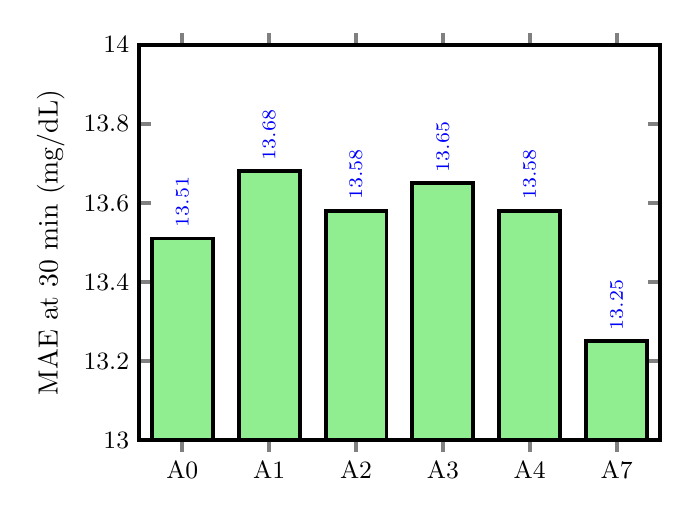
\begin{tikzpicture}
\begin{axis}[
  width=8.2cm, height=6.6cm,
  ybar,
  bar width=22pt,
  xlabel={},
  ylabel={MAE at 30 min (mg/dL)},
  symbolic x coords={A0,A1,A2,A3,A4,A7},
  xtick=data,
  ymin=13, ymax=14,
  axis line style={line width=1.4pt},
  tick style={line width=1.4pt},
  label style={font=\normalsize},
  tick label style={font=\small},
  nodes near coords,
  nodes near coords style={font=\scriptsize, color=blue, rotate=90, anchor=west},
  every node near coord/.append style={/pgf/number format/.cd, fixed, precision=2},
]

\addplot[
  fill={rgb,255:red,144;green,238;blue,144}, draw=black, line width=1.4pt,
] coordinates {
  (A0,13.51) (A1,13.68) (A2,13.58) (A3,13.65) (A4,13.58) (A7,13.25)
};

\end{axis}

\end{tikzpicture}
\caption{\small\textit{Point-accuracy ablation at 30 minutes comparing six physics configurations (A0-A4,A7), from no physics (A0) to full physics from epoch 1 (A7). A7 has the lowest MAE (13.25 mg/dL) versus 13.51 mg/dL for A0 in the primary run (seed 42). Multi-seed replication across 5 random seeds confirms this advantage is statistically significant across all horizons under paired Wilcoxon testing (Table~\ref{tab:multiseed}).}}
\label{fig:ablationfig}
\end{figure}

\subsubsection{Multi-Seed Replication and Statistical Significance}
\label{sec:multiseed_replication}

As a post hoc check of seed sensitivity, A0 and A7 were each retrained from scratch with five seeds $\{42, 101, 202, 303, 404\}$ under the official protocol. We report the mean and SD of MAE and RMSE across seeds, and paired two-sided Wilcoxon signed-rank tests on seed-averaged per-subject errors with Holm--Bonferroni correction (Table~\ref{tab:multiseed}).

\begin{table*}[t]
\centering
\caption{Post hoc multi-seed replication (5 seeds: 42, 101, 202, 303, 404) comparing A0 (no physics) and A7 (hybrid physics-guided), with paired Wilcoxon signed-rank tests on seed-averaged per-subject errors. Values are means over the five seeds and therefore differ from the single-seed (seed 42) values in Tables~\ref{tab:baselines_identical} and~\ref{tab:ablation}.}
\label{tab:multiseed}
\footnotesize
\setlength{\tabcolsep}{4.5pt}
\begin{tabular}{lrrrrrrrr}
\toprule
& \multicolumn{2}{c}{A0 (Transformer, no physics)} & \multicolumn{2}{c}{A7 (Hybrid physics-guided)} & \multicolumn{4}{c}{Paired Wilcoxon Test (Seed-Averaged)} \\
\cmidrule(lr){2-3} \cmidrule(lr){4-5} \cmidrule(lr){6-9}
Horizon & MAE ($\text{mean}\pm\text{SD}$) & RMSE ($\text{mean}\pm\text{SD}$) & MAE ($\text{mean}\pm\text{SD}$) & RMSE ($\text{mean}\pm\text{SD}$) & MAE Diff & $p_{\text{raw}}$ & $p_{\text{Holm}}$ & Significant? \\
\midrule
30 min & $13.88 \pm 0.25$ & $19.72 \pm 0.25$ & $\mathbf{13.37 \pm 0.11}$ & $\mathbf{19.17 \pm 0.16}$ & $-0.51$ & 0.00049 & 0.00195 & \textbf{Yes} ($p < 0.01$) \\
60 min & $23.78 \pm 0.64$ & $32.70 \pm 0.71$ & $\mathbf{22.60 \pm 0.32}$ & $\mathbf{31.23 \pm 0.44}$ & $-1.18$ & 0.00049 & 0.00195 & \textbf{Yes} ($p < 0.01$) \\
90 min & $31.21 \pm 1.00$ & $42.08 \pm 1.17$ & $\mathbf{29.28 \pm 0.53}$ & $\mathbf{39.61 \pm 0.70}$ & $-1.93$ & 0.00049 & 0.00195 & \textbf{Yes} ($p < 0.01$) \\
120 min & $36.46 \pm 1.07$ & $48.46 \pm 1.22$ & $\mathbf{34.08 \pm 0.64}$ & $\mathbf{45.47 \pm 0.86}$ & $-2.38$ & 0.00049 & 0.00195 & \textbf{Yes} ($p < 0.01$) \\
\bottomrule
\end{tabular}
\end{table*}

A7 significantly outperformed A0 at every horizon ($p_{\text{Holm}} = 0.00195$ for both MAE and RMSE), with an MAE advantage of 0.51~mg/dL at 30~min and 2.38~mg/dL at 120~min. Physics also reduced variability across seeds: the seed SD was 0.11 vs.\ 0.25~mg/dL at 30~min and 0.64 vs.\ 1.07~mg/dL at 120~min for A7 vs.\ A0.

\subsection{Clinical Accuracy and Hypoglycemia Detection}

Clinical agreement remains high across horizons: Clarke A+B decreases from 99.0\% at 30 minutes to 94.3\% at 120 minutes (Fig.~\ref{fig:clarke}). The Parkes error grid, pooled across test windows, shows the same pattern: zone A+B falls from 99.8\% at 30 minutes to 95.9\% at 120 minutes, and zone E is 0\% at every horizon.

Because Clarke and Parkes grids were designed for point-in-time sensor measurements rather than forecasts, we also applied Prediction Error Grid Analysis (PRED-EGA)~\cite{ref53}, which classifies predictions as Accurate, Benign, or Erroneous separately in hypoglycemia ($\le 70$~mg/dL, following the PRED-EGA definition), euglycemia (70--180~mg/dL), and hyperglycemia ($> 180$~mg/dL) (Table~\ref{tab:predega}). Clinically acceptable predictions (Accurate + Benign) exceeded 99.4\% at every horizon, and Erroneous predictions stayed below 0.6\% even at 120~min. In hyperglycemia, 96.2\% of predictions were Accurate at 30~min and 86.1\% at 60~min; in hypoglycemia, Erroneous predictions were 0.00\% at 30~min and 0.13\% at 60~min.

\begin{table*}[t]
\centering
\caption{PRED-EGA (Sivananthan et al.~\cite{ref53}) clinical prediction error grid results across 12 subjects (mean $\pm$ SD across subjects)}
\label{tab:predega}
\footnotesize
\begin{tabular}{lrrrr}
\toprule
Metric & 30 min & 60 min & 90 min & 120 min \\
\midrule
Overall Accurate (\%) & $90.8 \pm 3.3$ & $77.8 \pm 7.0$ & $68.6 \pm 8.1$ & $61.9 \pm 8.3$ \\
Overall Benign (\%) & $9.2 \pm 3.3$ & $21.9 \pm 7.0$ & $30.9 \pm 8.1$ & $37.5 \pm 8.2$ \\
Overall Erroneous (\%) & $0.04 \pm 0.07$ & $0.28 \pm 0.28$ & $0.50 \pm 0.39$ & $0.60 \pm 0.44$ \\
\textbf{Clinically Acceptable (\%)} & $\mathbf{99.96 \pm 0.07}$ & $\mathbf{99.72 \pm 0.28}$ & $\mathbf{99.50 \pm 0.39}$ & $\mathbf{99.40 \pm 0.44}$ \\
\midrule
Hypoglycemia Accurate (\%) & $65.9 \pm 20.1$ & $33.8 \pm 16.5$ & $18.3 \pm 12.0$ & $10.9 \pm 8.2$ \\
Hypoglycemia Erroneous (\%) & $0.00 \pm 0.00$ & $0.13 \pm 0.44$ & $0.24 \pm 0.54$ & $1.59 \pm 3.82$ \\
Hyperglycemia Accurate (\%) & $96.2 \pm 2.8$ & $86.1 \pm 6.8$ & $75.6 \pm 9.6$ & $66.1 \pm 12.0$ \\
Hyperglycemia Erroneous (\%) & $0.00 \pm 0.00$ & $0.00 \pm 0.00$ & $0.00 \pm 0.00$ & $0.00 \pm 0.00$ \\
\bottomrule
\end{tabular}
\end{table*}

However, as observed with Clarke zone A, standard point-forecast metrics reward predictions close to the center and can underestimate acute excursions. Thus, 89.8\% of predictions in Clarke zone A and 99.96\% in PRED-EGA clinically acceptable at 30 minutes can still coexist with the median point forecast missing 45\% of hypoglycemic readings (pointwise sensitivity 0.551; Table~\ref{tab:hypo_event}).

\pgfplotstableread[col sep=comma]{data/summary_model.csv}\summarytable
\pgfplotstablegetelem{0}{clarke_zone_A_pct_mean}\of\summarytable \global\let\ClAa=\pgfplotsretval
\pgfplotstablegetelem{1}{clarke_zone_A_pct_mean}\of\summarytable \global\let\ClAb=\pgfplotsretval
\pgfplotstablegetelem{2}{clarke_zone_A_pct_mean}\of\summarytable \global\let\ClAc=\pgfplotsretval
\pgfplotstablegetelem{3}{clarke_zone_A_pct_mean}\of\summarytable \global\let\ClAd=\pgfplotsretval
\pgfplotstablegetelem{0}{clarke_zone_B_pct_mean}\of\summarytable \global\let\ClBa=\pgfplotsretval
\pgfplotstablegetelem{1}{clarke_zone_B_pct_mean}\of\summarytable \global\let\ClBb=\pgfplotsretval
\pgfplotstablegetelem{2}{clarke_zone_B_pct_mean}\of\summarytable \global\let\ClBc=\pgfplotsretval
\pgfplotstablegetelem{3}{clarke_zone_B_pct_mean}\of\summarytable \global\let\ClBd=\pgfplotsretval
\pgfplotstablegetelem{0}{clarke_zone_C_pct_mean}\of\summarytable \global\let\ClCa=\pgfplotsretval
\pgfplotstablegetelem{1}{clarke_zone_C_pct_mean}\of\summarytable \global\let\ClCb=\pgfplotsretval
\pgfplotstablegetelem{2}{clarke_zone_C_pct_mean}\of\summarytable \global\let\ClCc=\pgfplotsretval
\pgfplotstablegetelem{3}{clarke_zone_C_pct_mean}\of\summarytable \global\let\ClCd=\pgfplotsretval
\pgfplotstablegetelem{0}{clarke_zone_D_pct_mean}\of\summarytable \global\let\ClDa=\pgfplotsretval
\pgfplotstablegetelem{1}{clarke_zone_D_pct_mean}\of\summarytable \global\let\ClDb=\pgfplotsretval
\pgfplotstablegetelem{2}{clarke_zone_D_pct_mean}\of\summarytable \global\let\ClDc=\pgfplotsretval
\pgfplotstablegetelem{3}{clarke_zone_D_pct_mean}\of\summarytable \global\let\ClDd=\pgfplotsretval
\pgfplotstablegetelem{0}{clarke_zone_E_pct_mean}\of\summarytable \global\let\ClEa=\pgfplotsretval
\pgfplotstablegetelem{1}{clarke_zone_E_pct_mean}\of\summarytable \global\let\ClEb=\pgfplotsretval
\pgfplotstablegetelem{2}{clarke_zone_E_pct_mean}\of\summarytable \global\let\ClEc=\pgfplotsretval
\pgfplotstablegetelem{3}{clarke_zone_E_pct_mean}\of\summarytable \global\let\ClEd=\pgfplotsretval

% ===================== FIG. 5 : Clarke error grid =====================
% Needs only \usepackage{pgfplots} in the preamble. Paste as-is.
\begin{figure}[!t]
\centering
\definecolor{pdBlue}{RGB}{0,96,173}
\definecolor{pdGreen}{RGB}{1,142,19}
\definecolor{pdRed}{RGB}{205,16,36}
\definecolor{pdPurple}{RGB}{148,101,181}
\definecolor{pdDeep}{RGB}{63,0,109}
\begin{tikzpicture}
\begin{axis}[
  width=\columnwidth, height=6.4cm,
  ybar stacked, bar width=20pt,
  xtick={30,60,90,120}, xtick pos=left, ytick pos=left,
  enlarge x limits=0.18,
  ymin=50, ymax=112, ytick={50,60,...,100},
  axis line style={line width=1.3pt, black},
  every tick/.style={black, line width=0.8pt},
  ymajorgrids, grid style={dashed, gray!35},
  tick label style={font=\footnotesize},
  label style={font=\footnotesize},
  xlabel={Horizon (min)}, ylabel={Clarke zone share (\%)},
  legend style={at={(0.5,0.975)}, anchor=north, legend columns=5,
                font=\scriptsize, draw=black!70, fill=white,
                /tikz/every even column/.append style={column sep=4pt}},
  legend image code/.code={\fill[#1] (0cm,-0.08cm) rectangle (0.28cm,0.14cm);},
]
\addplot[fill=pdGreen,  draw=none] coordinates {(30,89.8030) (60,75.3078) (90,64.8889) (120,57.9062)}; % A
\addplot[fill=pdBlue,   draw=none] coordinates {(30,9.1967)  (60,22.1306) (90,30.9045) (120,36.4372)}; % B
\addplot[fill=pdPurple, draw=none] coordinates {(30,0.0067)  (60,0.1263)  (90,0.4167)  (120,0.6412)};  % C
\addplot[fill=pdRed,    draw=none] coordinates {(30,0.9937)  (60,2.4307)  (90,3.7833)  (120,4.9732)};  % D
\addplot[fill=pdDeep,   draw=none] coordinates {(30,0.0000)  (60,0.0046)  (90,0.0067)  (120,0.0422)};  % E
\legend{A,B,C,D,E}
\end{axis}
\end{tikzpicture}
\caption{\small\textit{Clarke error-grid composition across 30/60/90/120-minute horizons. Zone A decreases from $\sim$90\% to $\sim$58\%, with the difference shifting mainly to zone B, while dangerous zones D and E remain negligible. Despite this favorable composition, the median forecast still misses many hypoglycemic events, so low D/E rates should not be interpreted as high hypoglycemia sensitivity.}}
\label{fig:clarke}
\end{figure}


\subsection{Hypoglycemia Detection and Predictive Distribution Calibration}

Point forecasts trained with squared or Huber losses regress toward the mean and underestimate hypoglycemic excursions. We therefore evaluated hypoglycemia detection in four ways: consensus event-level detection, a head-to-head comparison of A0 and A7 with quantile heads, validation-based threshold selection, and multi-horizon calibration.

\subsubsection{Consensus Event-Based Hypoglycemia Evaluation}
Following international consensus~\cite{ref52}, a hypoglycemic episode was defined as at least 15 continuous minutes (three consecutive 5-minute readings) below 70~mg/dL; the test set contains 56 such episodes over 92.0 patient-days (Table~\ref{tab:hypo_event}). The median forecast detected 11 of 56 events (sensitivity 19.6\%, specificity 99.4\%, 0.62 false alarms/day, median lead time 15~min). An alarm on the lower quantile ($\hat{G}_{0.10} < 70$~mg/dL) detected 38 of 56 before onset (67.9\%; specificity 95.4\%, 2.21 false alarms/day, median lead time 15~min). Monitoring $\min(\hat{G}_{0.10}(30), \hat{G}_{0.10}(60)) < 70$~mg/dL detected 46 of 56 (82.1\%; specificity 92.1\%, 3.46 false alarms/day) and extended the median lead time to 25.0~min.

\subsubsection{Quantile Alarm for Baseline A0 vs.\ Physics A7}
\label{sec:quantile_a0_a7}
To test whether physics worsens hypoglycemia detection when both models have quantile heads, A0 was retrained with the same non-crossing quantile head and compared with A7 (Table~\ref{tab:hypo_event}). With the median forecast, A7 had higher sensitivity than A0 (pointwise 0.551 vs.\ 0.413; event-level 19.6\% vs.\ 10.7\%) at similar specificity (99.3\% vs.\ 99.4\%). With the $q = 0.10$ alarm, A7 was again more sensitive (pointwise 0.918 vs.\ 0.861; event-level 67.9\% vs.\ 58.9\%) at comparable specificity (95.4\% vs.\ 95.9\%). In this comparison, physics does not degrade hypoglycemia detection.

\subsubsection{Validation Threshold Selection and Operating Curves}
\label{sec:validation_threshold_selection}
To avoid test-set reuse, the alarm threshold was chosen on the validation split by maximizing the $F_2$ score, which weights sensitivity twice as heavily as precision. The selected threshold, $T^* = 84.0$~mg/dL ($F_2 = 0.771$), was evaluated once on the test split. With true hypoglycemia ($G < 70$~mg/dL) as the target, alarming at $\hat{G}_{0.10} < 84$~mg/dL gave sensitivity 0.988, specificity 0.868, precision 0.175, and 3,397 false positives, compared with 0.918, 0.951, and 0.347 (1,257 false positives) for the standard 70~mg/dL alarm. If the target is also redefined as $G < 84$~mg/dL, the same alarm gives sensitivity 0.943, specificity 0.908, and precision 0.451. The higher threshold therefore trades precision for sensitivity. Sensitivity--precision curves for $q \in \{0.05, 0.10, 0.20\}$ (\texttt{data/sensitivity\_precision\_curves.csv}) show that the operating point can be adjusted along a continuous trade-off.

\begin{table*}[t]
\centering
\caption{Consensus event-level and pointwise hypoglycemia detection at 30 minutes across models and alarm heads (92.0 patient-days, 56 episodes). A0 was retrained with the same quantile head as A7 (Section~\ref{sec:quantile_a0_a7}), so its values differ from the single-seed ablation run in Table~\ref{tab:ablation}.}
\label{tab:hypo_event}
\footnotesize
\begin{tabular}{llrrrrrrr}
\toprule
Model & Alarm Head & \makecell{Point\\Sens.} & \makecell{Point\\Spec.} & \makecell{Point\\Prec.} & \makecell{Event\\Sens.} & Specificity & \makecell{False\\Alarms/Day} & \makecell{Median\\Lead Time} \\
\midrule
A0 (No physics) & Median (point) & 0.413 & 0.994 & 0.657 & 10.7\% & 99.4\% & 0.59 & 12.5 min \\
A0 (No physics) & Quantile $q=0.10$ & 0.861 & 0.956 & 0.357 & 58.9\% & 95.9\% & 2.00 & 15.0 min \\
\midrule
A7 (Physics hybrid) & Median (point) & 0.551 & 0.993 & 0.699 & 19.6\% & 99.4\% & 0.62 & 15.0 min \\
A7 (Physics hybrid) & Quantile $q=0.10$ & \textbf{0.918} & 0.951 & 0.347 & \textbf{67.9\%} & 95.4\% & 2.21 & 15.0 min \\
A7 (Physics hybrid) & Multi-horizon $q=0.10$ & -- & -- & -- & \textbf{82.1\%} & 92.1\% & 3.46 & \textbf{25.0 min} \\
\bottomrule
\end{tabular}
\end{table*}

\subsubsection{Calibration and Uncertainty Quantification}
Table~\ref{tab:calibration} reports calibration, sharpness, and scoring rules. Empirical coverage of the nominal 80\% interval ($[q_{0.10}, q_{0.90}]$) was 79.4\%, 78.5\%, 77.2\%, and 76.9\% at 30, 60, 90, and 120~min, and the lower quantile covered 9.47\% of observations at 30~min and 9.96\% at 120~min, close to the nominal 10.0\%. For glucose below 80~mg/dL, the interval covered 76.4\% of observations and the lower quantile 22.4\%. Between 30 and 120~min, mean interval width grew from 39.9 to 96.7~mg/dL and CRPS from 9.74 to 24.32~mg/dL.

\begin{table*}[t]
\centering
\caption{Multi-horizon calibration, conditional coverage, interval width, and scoring rules across all 12 subjects (26,498 test windows)}
\label{tab:calibration}
\footnotesize
\begin{tabular}{rrrrrrrrr}
\toprule
Horizon & \makecell{Nominal\\80\% Cov.} & \makecell{Lower\\$q_{0.10}$ Cov.} & \makecell{Upper\\$q_{0.90}$ Cov.} & \makecell{Cov.\\($G<80$)} & \makecell{Width\\(mg/dL)} & \makecell{Pinball\\($q_{0.10}$)} & \makecell{Pinball\\($q_{0.50}$)} & \makecell{CRPS\\(mg/dL)} \\
\midrule
30 min  & 79.4\% & 9.47\%  & 88.9\% & 76.4\% & 39.9 & 2.98 & 6.53  & 9.74 \\
60 min  & 78.5\% & 9.63\%  & 88.1\% & 64.1\% & 65.9 & 4.77 & 10.96 & 16.18 \\
90 min  & 77.2\% & 10.22\% & 87.4\% & 55.7\% & 83.2 & 6.02 & 14.17 & 20.85 \\
120 min & 76.9\% & 9.96\%  & 86.9\% & 53.3\% & 96.7 & 6.94 & 16.57 & 24.32 \\
\bottomrule
\end{tabular}
\end{table*}



Point forecasts also increasingly compress glucose excursions at longer horizons. The predicted-to-actual coefficient-of-variation ratio decreases from 0.973 to 0.802, with TIR increasingly overestimated and TBR underestimated (Fig.~\ref{fig:excursion}). Consistently, predicted LBGI falls increasingly below the actual value, from 0.65 versus 0.77 at 30 minutes to 0.33 versus 0.74 at 120 minutes, indicating progressively weaker representation of hypoglycemic risk in longer-horizon point forecasts.

\pgfplotstablegetelem{0}{actual_in_range_mean}\of\summarytable \global\let\tirActA=\pgfplotsretval
\pgfplotstablegetelem{1}{actual_in_range_mean}\of\summarytable \global\let\tirActB=\pgfplotsretval
\pgfplotstablegetelem{2}{actual_in_range_mean}\of\summarytable \global\let\tirActC=\pgfplotsretval
\pgfplotstablegetelem{3}{actual_in_range_mean}\of\summarytable \global\let\tirActD=\pgfplotsretval
\pgfplotstablegetelem{0}{predicted_in_range_mean}\of\summarytable \global\let\tirPredA=\pgfplotsretval
\pgfplotstablegetelem{1}{predicted_in_range_mean}\of\summarytable \global\let\tirPredB=\pgfplotsretval
\pgfplotstablegetelem{2}{predicted_in_range_mean}\of\summarytable \global\let\tirPredC=\pgfplotsretval
\pgfplotstablegetelem{3}{predicted_in_range_mean}\of\summarytable \global\let\tirPredD=\pgfplotsretval
\pgfplotstablegetelem{0}{actual_time_below_range_mean}\of\summarytable \global\let\tbrActA=\pgfplotsretval
\pgfplotstablegetelem{1}{actual_time_below_range_mean}\of\summarytable \global\let\tbrActB=\pgfplotsretval
\pgfplotstablegetelem{2}{actual_time_below_range_mean}\of\summarytable \global\let\tbrActC=\pgfplotsretval
\pgfplotstablegetelem{3}{actual_time_below_range_mean}\of\summarytable \global\let\tbrActD=\pgfplotsretval
\pgfplotstablegetelem{0}{predicted_time_below_range_mean}\of\summarytable \global\let\tbrPredA=\pgfplotsretval
\pgfplotstablegetelem{1}{predicted_time_below_range_mean}\of\summarytable \global\let\tbrPredB=\pgfplotsretval
\pgfplotstablegetelem{2}{predicted_time_below_range_mean}\of\summarytable \global\let\tbrPredC=\pgfplotsretval
\pgfplotstablegetelem{3}{predicted_time_below_range_mean}\of\summarytable \global\let\tbrPredD=\pgfplotsretval
\pgfplotstablegetelem{0}{cv_ratio_mean}\of\summarytable \global\let\cvA=\pgfplotsretval
\pgfplotstablegetelem{1}{cv_ratio_mean}\of\summarytable \global\let\cvB=\pgfplotsretval
\pgfplotstablegetelem{2}{cv_ratio_mean}\of\summarytable \global\let\cvC=\pgfplotsretval
\pgfplotstablegetelem{3}{cv_ratio_mean}\of\summarytable \global\let\cvD=\pgfplotsretval
% ============ FIG. 7 : Excursion compression (TIR / TBR / CV) ============
% Needs only \usepackage{pgfplots} in the preamble. Paste as-is.
% ============ FIG. 7 : Excursion compression (TIR / TBR / CV) ============
% Needs only \usepackage{pgfplots} in the preamble. Paste as-is.
\begin{figure*}[t]
\centering
\definecolor{pdBlue}{RGB}{0,96,173}
\definecolor{pdGreen}{RGB}{1,142,19}
\definecolor{pdRed}{RGB}{205,16,36}
\definecolor{pdPurple}{RGB}{148,101,181}
\pgfplotsset{f7/.style={
  scale only axis, width=0.68\linewidth, height=3.4cm,
  xtick={30,60,90,120}, xmin=20, xmax=130, xtick pos=left, ytick pos=left,
  axis line style={line width=1.3pt, black},
  every tick/.style={black, line width=0.8pt},
  ymajorgrids, grid style={dashed, gray!35},
  tick label style={font=\footnotesize},
  label style={font=\footnotesize},
  xlabel={Horizon (min)},
  legend style={font=\scriptsize, draw=black!70, fill=white},
  legend cell align=left,
  mark size=2.2pt, every axis plot/.append style={line width=1.2pt}}}
% ---- (a) TIR ----
\begin{minipage}[t]{0.325\textwidth}\centering
\begin{tikzpicture}
\begin{axis}[f7, ymin=60, ymax=76, ytick={60,64,...,76}, ylabel={TIR (\%)},
  legend pos=north west]
\addplot[color=pdBlue, mark=o]       coordinates {(30,62.3151) (60,62.1693) (90,62.1248) (120,62.1755)};
\addplot[color=pdRed,  mark=square*] coordinates {(30,63.8909) (60,67.7343) (90,70.5551) (120,73.1564)};
\legend{Actual,Predicted}
\end{axis}
\end{tikzpicture}\\[2pt]
{\normalsize\bfseries (a)}
\end{minipage}\hfill
% ---- (b) TBR ----
\begin{minipage}[t]{0.325\textwidth}\centering
\begin{tikzpicture}
\begin{axis}[f7, ymin=0, ymax=3.4, ytick={0,0.5,...,3}, ylabel={TBR (\%)},
  yticklabel style={/pgf/number format/fixed,/pgf/number format/precision=1},
  legend pos=south west]
\addplot[color=pdBlue, mark=o]       coordinates {(30,2.8617) (60,2.8444) (90,2.8210) (120,2.7881)};
\addplot[color=pdRed,  mark=square*] coordinates {(30,2.3059) (60,1.3630) (90,0.8491) (120,0.6079)};
\legend{Actual,Predicted}
\end{axis}
\end{tikzpicture}\\[2pt]
{\normalsize\bfseries (b)}
\end{minipage}\hfill
% ---- (c) CV ratio ----
\begin{minipage}[t]{0.325\textwidth}\centering
\begin{tikzpicture}
\begin{axis}[f7, ymin=0.75, ymax=1.05, ytick={0.75,0.80,...,1.05}, ylabel={CV ratio},
  yticklabel style={/pgf/number format/fixed,/pgf/number format/precision=2,
                    /pgf/number format/fixed zerofill},
  legend pos=south west]
\addplot[color=pdPurple, mark=triangle*]       coordinates {(30,0.9725) (60,0.9010) (90,0.8413) (120,0.8023)};
\addplot[color=pdGreen, dashed, mark=diamond*] coordinates {(30,1) (60,1) (90,1) (120,1)};
\legend{CV ratio,Reference (=1)}
\end{axis}
\end{tikzpicture}\\[2pt]
{\normalsize\bfseries (c)}
\end{minipage}
\caption{\small\textit{Excursion compression with horizon (30/60/90/120 minutes). a: actual time-in-range (TIR) stays flat near 62\% while predicted TIR climbs toward 74\%, an increasing overestimate. b: actual time-below-range (TBR) stays flat near 2.8\% while predicted TBR falls toward 0.6\%, an increasing underestimate of hypoglycemic exposure. c: the predicted-to-actual coefficient-of-variation ratio declines from about 0.97 to 0.80. All three panels show the same mechanism: as the horizon lengthens, the point forecast increasingly regresses toward the mean and loses the variance of the true glucose trace.}}
\label{fig:excursion}
\end{figure*}




\subsection{Patient-Specific Insulin Sensitivity and Physiological Validation}
\label{sec:si_validation}

Three preregistered checks determine whether $S_I$ may be interpreted physiologically (Table~\ref{tab:si}). All pass under the official protocol: between-subject variation is non-degenerate ($\text{CV} = 35.8\%$), test--retest reliability is high ($\text{ICC}(1) = 0.890$), and $S_I$ is strongly inversely related to total daily insulin dose ($\rho = -0.839$, 95\% CI [$-0.99, -0.44$]). Under LOSO, stability and variability remain, but the dose correlation fails. Hence $S_I$ is a stable, subject-specific estimate with external validity demonstrated only in the personalized setting; cross-subject validity is not established.

\begin{table}[t]
\centering
\caption{Preregistered validation of insulin sensitivity}
\label{tab:si}
\footnotesize
\resizebox{\columnwidth}{!}{%
\begin{tabular}{lrrr}
\toprule
Check & Threshold & Official & LOSO \\
\midrule
Between-subject CV & $>$10\% & 35.8\% & 34.3\% \\
Test--retest ICC(1) & $>$0.5 & 0.890 & 0.816 \\
$\rho$ vs.\ total daily dose & $<$0, CI excludes 0 & $-0.839$ & $-0.357$ \\
95\% CI for $\rho$ & -- & [$-0.99$, $-0.44$] & [$-0.82$, $0.28$] \\
\bottomrule
\end{tabular}%
}
\end{table}

\subsubsection{Addressing Potential Circularity and Confounding}
We tested whether the stability and dose correlation of $S_I$ could be artifacts of the temporal-consistency loss or of ambient glucose, and whether $S_I$ agrees with classical minimal-model estimation (Table~\ref{tab:si_circularity}):

\begin{enumerate}
    \item \textbf{No temporal-consistency loss ($\lambda_{tc} = 0$):} Retrained without the penalty (\texttt{abl-A7-notc}), $S_I$ still passed all checks: ICC(1) = 0.645, CV = 22.2\%, all estimates within the Ward IDDM bounds, and $\rho = -0.804$ with total daily dose ($p = 0.0016$, 95\% CI [$-0.955, -0.451$]). Stability is therefore not produced solely by the penalty.
    \item \textbf{Partial correlation controlling for mean glucose:} Controlling for test-interval mean glucose, the $S_I$--TDD partial correlation was $r = -0.838$ (rank, $p = 0.0013$) and $r = -0.886$ (Pearson, $p = 0.0003$); controlling for whole-study mean glucose gave $r = -0.843$ ($p = 0.0011$) and $r = -0.875$ ($p = 0.0004$). Ambient glucose does not explain the relationship.
    \item \textbf{Independent minimal-model fit:} $S_I$ from the parameter head agreed with per-subject Bergman estimates obtained by nonlinear least squares/MAP (Spearman $\rho = 0.790$, $p = 0.0022$; Pearson $r = 0.831$, $p = 0.0008$), without iterative fitting at inference.
    \item \textbf{Insulin-to-carbohydrate ratio:} For the six 2018 subjects with clinical ICR (grams of carbohydrate per unit of insulin, so a positive correlation is expected), the correlation with $S_I$ was Spearman $\rho = +0.371$ ($p = 0.469$) and Pearson $r = +0.079$ ($p = 0.881$); with $n = 6$, this check is underpowered.
    \item \textbf{Learned trust gate $g$:} The gate on the Bergman prior, initialized at $g_0 \approx 0.10$, converged to 0.152 in the point forecaster (A7) and 0.128 in the quantile forecaster.
\end{enumerate}

\begin{table*}[t]
\centering
\caption{Non-circularity, confounding, and physiological validation of learned insulin sensitivity $S_I$}
\label{tab:si_circularity}
\footnotesize
\begin{tabular}{lrr}
\toprule
Analysis / Validation Check & Value & Interpretation / Threshold \\
\midrule
\multicolumn{3}{l}{\textit{Temporal Consistency Ablation ($\lambda_{tc} = 0.0$):}} \\
Between-subject CV & 22.2\% & Non-degenerate ($> 10\%$) \\
Test--retest reliability ICC(1) & 0.645 & Stable without penalty ($> 0.5$) \\
Spearman $\rho$ vs.\ TDD & $-0.804$ & Significant ($p=0.0016$, 95\% CI [$-0.96, -0.45$]) \\
Ward IDDM range adherence & 100\% & Within bounds (partly imposed by design) \\
\midrule
\multicolumn{3}{l}{\textit{Confounding by Ambient Glucose:}} \\
Unadjusted $\rho(S_I, \text{TDD})$ & $-0.839$ & Baseline ($p = 0.0006$) \\
Partial rank $r(S_I, \text{TDD} \mid \bar{G}_{\text{test}})$ & $-0.838$ & After adjustment ($p = 0.0013$) \\
Partial Pearson $r(S_I, \text{TDD} \mid \bar{G}_{\text{test}})$ & $-0.886$ & After adjustment ($p = 0.0003$) \\
Partial rank $r(S_I, \text{TDD} \mid \bar{G}_{\text{all}})$ & $-0.843$ & After adjustment ($p = 0.0011$) \\
\midrule
\multicolumn{3}{l}{\textit{External Validation against Classic Minimal Model:}} \\
Agreement with NLS/MAP Bergman (Spearman $\rho$) & $+0.790$ & Agreement ($p = 0.0022$) \\
Agreement with NLS/MAP Bergman (Pearson $r$) & $+0.831$ & Agreement ($p = 0.0008$) \\
Agreement with clinical ICR ($n=6$, exploratory) & $+0.371$ & Underpowered ($p = 0.469$) \\
\midrule
\multicolumn{3}{l}{\textit{Mechanistic Prior Trust Gate:}} \\
Initialized gate $g_0 = \sigma(-2.2)$ & 9.98\% & Initialization \\
Converged gate $g$ (Point Forecaster, A7) & 15.2\% & Converged value \\
Converged gate $g$ (Quantile Forecaster, A7) & 12.8\% & Converged value \\
\bottomrule
\end{tabular}
\end{table*}

Body weight is not identifiable because all OhioT1DM files use the same de-identification placeholder. The dose-per-kilogram correlation is therefore not independent of total daily dose. Moreover, $p_2$ and $p_3$ are range-constrained, so agreement with a plausible interval is partly imposed rather than learned.

\subsection{Feature Attribution}
\label{sec:attribution}

IG and permutation importance agree with Spearman $\rho = 0.731$ ($p = 6.05 \times 10^{-7}$, $n=35$) and share three of their top five features. Both rank five-minute glucose rate of change first by a wide margin. Permuting it raises MAE by 3.11 mg/dL, over seven times the next feature. The group-level IG result in Fig.~\ref{fig:attribution} assigns 42.7\% to glucose-derived features and 27.1\% to mechanistic states, showing that physiology-derived inputs are informative in their own right.

Attribution concentrates in the most recent input positions, supporting attention pooling. The IG completeness discrepancy has median relative magnitude 3.2\% and $p_{95}$ 70\%; it does not shrink with more integration steps and remains unresolved. Conclusions are therefore restricted to findings corroborated by permutation importance.

\pgfplotstableread[col sep=comma]{data/integrated_gradients_by_group_30min.csv}\igtable
\pgfplotstablegetelem{0}{share_pct}\of\igtable \global\let\igGlu=\pgfplotsretval
\pgfplotstablegetelem{1}{share_pct}\of\igtable \global\let\igMech=\pgfplotsretval
\pgfplotstablegetelem{2}{share_pct}\of\igtable \global\let\igTher=\pgfplotsretval
\pgfplotstablegetelem{3}{share_pct}\of\igtable \global\let\igTime=\pgfplotsretval
\pgfplotstablegetelem{4}{share_pct}\of\igtable \global\let\igSens=\pgfplotsretval
\pgfplotstablegetelem{5}{share_pct}\of\igtable \global\let\igCtx=\pgfplotsretval
\pgfplotstableread[col sep=comma]{data/permutation_importance_30min.csv}\pitable
% rows 0-8, in file order, are exactly the true top-9 by mae_increase (descending).
\pgfplotstablegetelem{0}{mae_increase}\of\pitable \global\let\pmA=\pgfplotsretval % roc_5min
\pgfplotstablegetelem{1}{mae_increase}\of\pitable \global\let\pmB=\pgfplotsretval % roc_30min
\pgfplotstablegetelem{2}{mae_increase}\of\pitable \global\let\pmC=\pgfplotsretval % minutes_since_bolus
\pgfplotstablegetelem{3}{mae_increase}\of\pitable \global\let\pmD=\pgfplotsretval % is_night
\pgfplotstablegetelem{4}{mae_increase}\of\pitable \global\let\pmE=\pgfplotsretval % glucose_mean_1h
\pgfplotstablegetelem{5}{mae_increase}\of\pitable \global\let\pmF=\pgfplotsretval % glucose_mean_2h
\pgfplotstablegetelem{6}{mae_increase}\of\pitable \global\let\pmG=\pgfplotsretval % glucose_std_1h
\pgfplotstablegetelem{7}{mae_increase}\of\pitable \global\let\pmH=\pgfplotsretval % roc_15min
\pgfplotstablegetelem{8}{mae_increase}\of\pitable \global\let\pmI=\pgfplotsretval % hour_sin

% ============ FIG. 8 : Feature attribution (IG + permutation) ============
% Needs only \usepackage{pgfplots} in the preamble. Paste as-is.
\begin{figure*}[t]
\centering
\definecolor{pdBlue}{RGB}{0,96,173}
\definecolor{pdRed}{RGB}{205,16,36}
\pgfplotsset{f8/.style={
  scale only axis, height=3.6cm, xtick pos=left, ytick pos=left,
  axis line style={line width=1.3pt, black},
  every tick/.style={black, line width=0.8pt},
  grid style={dashed, gray!35},
  tick label style={font=\footnotesize},
  label style={font=\footnotesize}}}
% ---- (a) Integrated gradients by feature group ----
\begin{minipage}[t]{0.40\textwidth}\centering
\begin{tikzpicture}
\begin{axis}[f8, width=0.62\linewidth,
  xbar, bar width=9pt, xmajorgrids,
  ytick={0,1,2,3,4,5},
  yticklabels={Context,Sensor,Time,Therapy,Mechanistic,Glucose},
  ymin=-0.6, ymax=5.6,
  xmin=0, xmax=62, xtick={0,10,...,50},
  xlabel={IG share (\%)},
  nodes near coords={\pgfmathprintnumber[fixed,fixed zerofill,precision=1]{\pgfplotspointmeta}\%},
  nodes near coords style={font=\scriptsize, anchor=west, xshift=1pt},
  point meta=x]
\addplot[fill=pdBlue, draw=none] coordinates
  {(1.6582,0) (7.0079,1) (8.0782,2) (13.5090,3) (27.0757,4) (42.6710,5)};
\end{axis}
\end{tikzpicture}\\[2pt]
{\normalsize\bfseries (a)}
\end{minipage}\hfill
% ---- (b) Permutation importance (top 9 features) ----
\begin{minipage}[t]{0.57\textwidth}\centering
\begin{tikzpicture}
\begin{axis}[f8, width=0.62\linewidth,
  xbar, bar width=6.5pt, xmajorgrids,
  ytick={0,1,2,3,4,5,6,7,8},
  yticklabels={hour\_sin,roc\_15min,glucose\_std\_1h,glucose\_mean\_2h,glucose\_mean\_1h,is\_night,minutes\_since\_bolus,roc\_30min,roc\_5min},
  y tick label style={font=\scriptsize\ttfamily},
  ymin=-0.6, ymax=8.6,
  xmin=0, xmax=3.4, xtick={0,0.5,...,3},
  xticklabel style={/pgf/number format/fixed},
  xlabel={Permutation MAE increase (mg/dL)}]
\addplot[fill=pdRed, draw=none] coordinates
  {(0.2270,0) (0.2330,1) (0.2516,2) (0.2963,3) (0.3214,4) (0.3396,5) (0.4022,6) (0.4278,7) (3.1131,8)};
\end{axis}
\end{tikzpicture}\\[2pt]
{\normalsize\bfseries (b)}
\end{minipage}
\caption{\small\textit{Feature attribution at 30 min using integrated gradients (a) and permutation importance (b). Glucose-derived features dominate IG attribution (42.7\%), while \textnormal{\texttt{roc\_5}} is the strongest permuted feature ($\sim$3.1~mg/dL MAE increase). Both methods identify glucose dynamics as the leading predictors.}}
\label{fig:attribution}
\end{figure*}


\subsection{Comparison With Published Work}

At 30 minutes, the current work is mid-field relative to the 2020 challenge literature~\cite{ref64}, [\hyperref[ref60label]{70}-\hyperref[ref63label]{73}] (Table~\ref{tab:published}): on the matched 2020 cohort (subjects 540/544/552/567/584/596, the six subjects on which the challenge entries were scored), RMSE is 18.74 and MAE is 13.24~mg/dL. Further 2020 entries report RMSE@30 of 18.34 and 19.60~mg/dL~[\hyperref[ref65label]{74}-\hyperref[ref70label]{75}]. At 60 minutes, RMSE (31.16) is essentially tied with the best entry (31.10), and MAE (22.55) is lower than every entry except one whose MAE-to-RMSE ratio is far outside the range of the other entries~\cite{ref60}; differences in window eligibility, missing-data handling, external pretraining, and best-configuration reporting prevent a state-of-the-art claim. Across all 12 subjects, the only published comparison is GARNN~\cite{ref75} (18.97/13.34~mg/dL at 30 minutes), against which the all-subject result (18.84/13.08) should be read as a tie. The defensible advances are calibrated hypoglycemia detection, explicit personalized-versus-LOSO decomposition, preregistered validation of a physiological parameter, and a quantified account of the benefits and costs of Bergman constraints. The all-12-subject official figures reported throughout the Results section (e.g., 18.84/13.08 at 30 minutes) differ slightly from the 2020-cohort figures in Tables~\ref{tab:landscape} and~\ref{tab:published}; both are correct, answer different comparability questions, and should not be averaged together.

\begin{table*}[t]
\centering
\caption{Published OhioT1DM Comparison, 2020 Challenge Cohort ($\mathrm{mg/dL}$)}
\label{tab:published}
\footnotesize
\begin{tabular}{lrrrrrrrr}
\toprule
Method & R30 & A30 & R60 & A60 & R90 & A90 & R120 & A120 \\
\midrule
Freiburghaus CNN/LSTM~\cite{ref63} & 17.45 & 11.22 & 33.67 & 23.25 & -- & -- & -- & -- \\
Rubin-Falcone N-BEATS+BiLSTM~\cite{ref62} & 18.22 & 12.83 & 31.66 & 23.60 & -- & -- & -- & -- \\
Bevan--Coenen LSTM~\cite{ref61} & 18.23 & 14.37 & 31.10 & 25.75 & -- & -- & -- & -- \\
Pavan NN-EIM~\cite{ref60} & 18.63 & 10.08 & 32.27 & 17.69 & -- & -- & -- & -- \\
Yang MS-LSTM~\cite{ref64} & 19.05 & 13.50 & 32.03 & 23.83 & -- & -- & -- & -- \\
\textbf{Current Work, official} & \textbf{18.74} & \textbf{13.24} & \textbf{31.16} & \textbf{22.55} & \textbf{39.52} & \textbf{29.14} & \textbf{45.39} & \textbf{34.03} \\
Current Work, LOSO & 20.93 & 14.98 & 34.55 & 25.45 & 43.50 & 32.69 & 49.36 & 37.76 \\
Persistence & 24.22 & 17.45 & 40.11 & 29.51 & 51.15 & 38.34 & 58.98 & 44.83 \\
\bottomrule
\end{tabular}

\vspace{2pt}
\raggedright\footnotesize
--: not reported; the Blood Glucose Level Prediction (BGLP) Challenge required only 30- and 60-minute forecasts. Current Work and Persistence rows use the same six 2020-cohort subjects as the published entries; all-12-subject results are in Table~\ref{tab:official}.
\end{table*}




%=================================================================
\section{Discussion}

The results separate three concepts that are often conflated in digital-twin and glucose-prediction literature~\cite{ref2}. First, a mechanistic constraint can be useful beyond point accuracy. Here it improves accuracy only modestly (0.51--2.38~mg/dL MAE across horizons over five seeds), but it also supplies interpretable state variables and a stable $S_I$ estimate, and mechanistic features account for more than one quarter of total IG attribution. Second, a favorable error grid does not demonstrate event safety. The median forecast has excellent Clarke A+B coverage but inadequate hypoglycemia sensitivity; a calibrated predictive tail is required. Third, personalized temporal validation and cross-subject generalization answer different questions. The growing official--LOSO gap shows that access to a subject's history matters increasingly at longer horizons. Prospective digital-twin trials demonstrate the longer-term potential of individualized replay and adaptation, but do not remove the need to validate the forecasting layer independently~\cite{ref18}.

The ablation also exposes a structural limitation. Bergman's equilibrium at $G_b$ pulls trajectories toward the center of the glucose distribution. In the best configuration this adds approximately 1.3 mg/dL to an already-present regression-to-the-mean bias during hypoglycemia. This behavior appears whether physics enters as a penalty or a prior. A future model should modify the physiological structure rather than hide the bias with an asymmetric point loss.

%=================================================================
\section{Limitations and Future Work}

The cohort contains only 12 subjects and approximately 2,800 effectively independent observations. The ablation screen used a single seed (42); only A0 and A7 were replicated over five seeds, post hoc (Section~\ref{sec:multiseed_replication}). OhioT1DM has no clamp measurement of $S_I$, so validation is indirect; LOSO external validity fails. Subject 552 has only 59.7\% test CGM coverage, and subject 567 has no carbohydrate records in the test interval. Body weight is unavailable. The alarm operating point was selected on validation data without test-set reuse (Section~\ref{sec:validation_threshold_selection}), but lacks an elicited clinical cost ratio. No counterfactual intervention is validated, so the system is a physics-guided forecaster rather than a digital twin or treatment simulator.

The parameter head estimates a ten-component physiological vector $\theta_p$ for each subject, rather than only $S_I$. Table~\ref{tab:params} lists its components: $p_1$, $p_2$, $p_3$, $n$, $V_G$, $V_I$, $t_{\max,I}$, $k_{\text{gri}}$, $k_{\text{abs}}$, and $f$.

Preregistered external validation (Table~\ref{tab:si} and Table~\ref{tab:si_circularity}) was carried out for $S_I$ alone, for three concrete reasons rather than by omission. First, $S_I$ is the one component with a direct clinical measurement analogue: a euglycemic clamp measures exactly this quantity, giving a real external target to validate against, whereas the remaining parameters have no equivalent bedside measurement available in OhioT1DM\@. Second, $S_I$ has literature-sourced plausible bounds specific to insulin-dependent diabetes~\cite{ref33}, giving its sigmoid-mapped range a population anchor that is not equally well established for every other compartment parameter. Third, the ablation (Table~\ref{tab:ablation}, A3 vs.\ A4) already shows that per-patient parameter estimation is accuracy-neutral overall (0.07--0.76 mg/dL), so the contribution claimed here is the external validity of one physiological quantity, not evidence that the other nine are unimportant. One concrete obstacle already blocks part of this extension: body weight is unavailable because every OhioT1DM file carries the same de-identification placeholder, which is why a body-weight-normalized analysis was not attempted for any parameter, not only $S_I$.

Priority extensions are external validation on larger cohorts (e.g., Shanghai, DiaTrend), formal identifiability analysis of the remaining patient parameters, preregistered validation of the remaining Bergman and absorption parameters ($p_1, n, V_G, V_I$) against literature-sourced population anchors comparable to those used for $S_I$, time-varying $S_I$, a joint multi-horizon predictive distribution, decision-theoretic alarm selection with patient-specific cost matrices, longer context, and prospective validation of counterfactual meal and insulin interventions.

%=================================================================
\section{Conclusion}
\begin{table*}[t]
\centering
\caption{Patient-parameter vector $\theta_p$ and admissible intervals}
\label{tab:params}
\footnotesize
\begin{tabular}{clllr}
\toprule
Symbol & Meaning & Range & Unit & Population anchor \\
\midrule
$p_1$ & Insulin-independent glucose disposal & 0--0.030 & min$^{-1}$ & 0.013 \\
$p_2$ & Decay of remote insulin action & 0.005--0.10 & min$^{-1}$ & 0.025 \\
$p_3$ & Build rate of action from insulin excess & $10^{-6}$--$3\times10^{-5}$ & mL $\mu$U$^{-1}$min$^{-2}$ & $6.25\times10^{-6}$ \\
$n$ & Plasma insulin clearance & 0.08--0.25 & min$^{-1}$ & 0.138 \\
$V_G$ & Glucose distribution volume & 1.4--2.4 & dL/kg & 1.88 \\
$V_I$ & Insulin distribution volume & 0.08--0.18 & L/kg & 0.12 \\
$t_{\max,I}$ & Time to peak SC absorption & 30--90 & min & 55 \\
$k_{\text{gri}}$ & Gastric emptying rate & 0.008--0.10 & min$^{-1}$ & 0.035 \\
$k_{\text{abs}}$ & Intestinal absorption rate & 0.005--0.10 & min$^{-1}$ & 0.0167 \\
$f$ & Carbohydrate bioavailability & 0.70--1.00 & dimensionless & 0.90 \\
\bottomrule
\end{tabular}
\end{table*}

An audited, hybrid physics-guided forecaster can outperform a validated persistence baseline by 19--21\% RMSE across 30--120-minute horizons. Physics improves point accuracy only modestly, and significantly only in a post hoc five-seed replication. The strongest evidence is instead that physiology can provide stable patient-specific structure alongside this small accuracy gain, and that calibrated distributional forecasting can recover hypoglycemic events missed by an otherwise accurate median forecast. Horizon integrity, subject-level statistics, matched generalization protocols, and explicit safety trade-offs are prerequisites for credible glucose forecasting.

\newpage\null\newpage
%=================================================================
\appendices
\section{Notation, Variables, and Terminology}

This appendix summarizes the notation and feature groups used in the manuscript; full notation tables, including abbreviations, are in the Supplementary Material. Rate constants are expressed per minute unless stated otherwise. A subscript $b$ denotes a basal or fasting quantity, a hat denotes a prediction, bold lowercase symbols denote vectors, and bold uppercase symbols denote matrices.

\subsection{Physiological States and Inputs}

Glucose $G$ is propagated separately from a six-state linear compartment model. Insulin on board and carbohydrate on board are derived identities, not additional fitted states (cf.\ Eqs.~\eqref{eq:6}--\eqref{eq:7}, \eqref{eq:9}--\eqref{eq:10}):
\begin{equation}
\text{IOB} = S_1 + S_2, \qquad \text{COB} = Q_{\text{sto}} + Q_{\text{gut}}.
\label{eq:19}
\end{equation}

\subsection{Estimated Physiological Parameters}

The parameter head emits unconstrained values $z_i$, which are mapped to admissible, physiologically sourced intervals~\cite{ref33} by
\begin{equation}
\theta_i = \ell_i + (u_i - \ell_i)\sigma(z_i).
\label{eq:20}
\end{equation}

The bounds prevent nonphysical values but also mean that plausible range alone cannot establish identifiability.

The reported derived quantity is
\begin{equation}
S_I = p_3/p_2,
\label{eq:21}
\end{equation}
the steady-state gain from plasma insulin above basal to remote insulin action, already introduced as Eq.~\eqref{eq:5}~\cite{ref1,ref32}. Higher $S_I$ means a given insulin excess produces stronger glucose disposal. It is validated as a subject-specific estimate only when its cross-subject variation, test--retest ICC, and dose correlation meet the preregistered criteria.

The implementation-level objective, following Eq.~\eqref{eq:17}, can be written more explicitly as
\begin{equation}
\mathcal{L} = \mathcal{L}_{\text{Huber}} + \lambda_q \mathcal{L}_{\text{pinball}} + w_{\text{phys}} \mathcal{L}_{\text{res}} + \lambda_{\text{pr}} \mathcal{L}_{\text{prior}} + \lambda_{\text{tc}} \mathcal{L}_{\text{temporal}}.
\label{eq:22}
\end{equation}

\subsection{Feature Contract}

The 35-input feature contract contains six groups: nine glucose features (current glucose, three rates of change, and rolling summaries); nine mechanistic features (IOB, COB, the six compartment states, and glucose appearance); four therapy/timing features; three cyclic-time features; six sensor values or availability masks; and four behavioral/context indicators. Glucose features account for 42.7\% of IG magnitude, mechanistic features 27.1\%, therapy 13.5\%, time 8.1\%, sensors 7.0\%, and context 1.7\%. Every sensor channel has an availability indicator so missingness is not represented as a physiologically extreme standardized zero. Input interpolation is explicitly flagged, whereas forecast targets are always real CGM observations.

Table~\ref{tab:params} lists the estimated patient-parameter vector. Notation tables for physiological states and inputs, architecture, discretization and uncertainty, training losses, evaluation metrics, and abbreviations are provided in the Supplementary Material.












\mbox{}\par
\clearpage
%=================================================================
\makeatletter\global\@colroom=\@colht \global\vsize=\@colht\makeatother
\begin{thebibliography}{99}
\sloppy
\setlength{\itemsep}{1.5pt}

\bibitem{ref1}\label{ref1label} R.~N. Bergman, Y.~Z. Ider, C.~R. Bowden, and C. Cobelli, ``Quantitative estimation of insulin sensitivity,'' \emph{Am. J. Physiol.}, vol. 236, no. 6, pp. E667--E677, 1979.

\bibitem{ref2}\label{ref2label} G. Cappon and A. Facchinetti, ``Digital twins in type 1 diabetes: A systematic review,'' \emph{J. Diabetes Sci. Technol.}, vol. 19, no. 1, 2025.

\bibitem{ref19}\label{ref19label} E. Acu\~{n}a and R. Aparicio, ``Predicting the blood glucose level using transformers,'' in \emph{Proc. 2023 Int. Conf. Computational Science and Computational Intelligence (CSCI)}, 2023, pp. 1392--1399, doi: 10.1109/CSCI62032.2023.00228.

\bibitem{ref20}\label{ref20label} A. Marx, F. Di Stefano, H. Leutheuser, K. Chin-Cheong, M. Pfister, M.-A. Burckhardt, S. Bachmann, and J.~E. Vogt, ``Blood glucose forecasting from temporal and static information in children with T1D,'' \emph{Front. Pediatr.}, vol. 11, Art. no. 1296904, 2023, doi: 10.3389/fped.2023.1296904.

\bibitem{ref21}\label{ref21label} Q. Bian, A. As'arry, X. Cong, K.~A. Md Rezali, and R.~M.~K. Raja Ahmad, ``A hybrid Transformer-LSTM model applied to glucose prediction,'' \emph{PLOS ONE}, vol. 19, no. 9, Art. no. e0310084, 2024.

\bibitem{ref22}\label{ref22label} X. Xiong, X. Yang, Y. Cai, Y. Xue, J. He, and H. Su, ``Exploring the potential of deep learning models integrating transformer and LSTM in predicting blood glucose levels for T1D patients,'' \emph{Digit. Health}, vol. 11, Art. no. 20552076251328980, 2025, doi: 10.1177/20552076251328980.

\bibitem{ref3}\label{ref3label} C. Duckworth, M.~J. Guy, \emph{et al.}, ``Explainable machine learning for real-time hypoglycemia and hyperglycemia prediction and personalized control recommendations,'' \emph{J. Diabetes Sci. Technol.}, vol. 18, no. 1, 2024.

\bibitem{ref5}\label{ref5label} S.~L. Cichosz, S.~S. Olesen, and M.~H. Jensen, ``Explainable machine-learning models to predict weekly risk of hyperglycemia, hypoglycemia, and glycemic variability in patients with type 1 diabetes based on continuous glucose monitoring,'' \emph{J. Diabetes Sci. Technol.}, vol. 20, no. 3, pp. 836--847, 2024.

\bibitem{ref8}\label{ref8label} M. Raissi, P. Perdikaris, and G.~E. Karniadakis, ``Physics-informed neural networks: A deep learning framework for solving forward and inverse problems involving nonlinear partial differential equations,'' \emph{J. Comput. Phys.}, vol. 378, pp. 686--707, 2019.

\bibitem{ref9}\label{ref9label} R. Pei and W. Wang, ``PINN based short-term glucose prediction for type 1 diabetes,'' in \emph{2025 4th Asia Conf. Algorithms, Computing and Machine Learning (CACML)}, Guangzhou, China, 2025, pp. 1--6.

\bibitem{ref10}\label{ref10label} M. Wang, H. Zhang, and R. Song, ``Blood glucose prediction algorithm via PINN under Bergman's Minimal Model constraints,'' in \emph{2025 IEEE 14th Data Driven Control and Learning Systems Conf. (DDCLS)}, Wuxi, China, 2025, pp. 1797--1802.

\bibitem{ref11}\label{ref11label} W. Wang, R. Pei, D. Li, S. Liu, Y. Geng, and S. Wang, ``A physics-informed glucose-insulin neural network model for glucose prediction,'' \emph{Tsinghua Sci. Technol.}, 2026.

\bibitem{ref12}\label{ref12label} P.~A. Mongini, M. Drecogna, and C. Toffanin, ``New physics-LSTM hybrid models for control-oriented glucose prediction in Type 1 Diabetes,'' in \emph{2025 American Control Conf. (ACC)}, Denver, CO, USA, 2025, pp. 662--667.

\bibitem{ref13}\label{ref13label} P. Colmegna, K. Wang, J. Garcia-Tirado, and M.~D. Breton, ``Mapping data to virtual patients in type 1 diabetes,'' \emph{Control Eng. Pract.}, vol. 103, Art. no. 104605, 2020, doi: 10.1016/j.conengprac.2020.104605.

\bibitem{ref14}\label{ref14label} G. Cappon, M. Vettoretti, G. Sparacino, S. Del Favero, and A. Facchinetti, ``ReplayBG: A digital twin-based methodology to identify a personalized model from type 1 diabetes data and simulate glucose concentrations to assess alternative therapies,'' \emph{IEEE Trans. Biomed. Eng.}, vol. 70, no. 11, pp. 3227--3238, 2023, doi: 10.1109/TBME.2023.3286856.

\bibitem{ref16}\label{ref16label} V. Roquemen-Echeverri, T. Kushner, P.~G. Jacobs, and C. Mosquera-Lopez, ``A physiologically-constrained neural network digital twin framework for replicating glucose dynamics in type 1 diabetes,'' \emph{Neural Comput. Appl.}, vol. 38, p. 241, 2026.

\bibitem{ref17}\label{ref17label} C.~E. Builes-Monta\~no, L. Lema-Perez, A. Ram\'{\i}rez-Rinc\'on, J.~J. Zuleta-Tob\'on, J.~C. Restrepo-Guti\'errez, H.~D. \'Alvarez-Zapata, J. Garc\'{\i}a-Tirado, \emph{et al.}, ``A digital twin-enhanced decision support system improves time-in-range in type 1 diabetes: a randomised clinical trial,'' \emph{Sci. Rep.}, vol. 15, Art. no. 39738, 2025, doi: 10.1038/s41598-025-23165-x.

\bibitem{ref18}\label{ref18label} B. Kovatchev, P. Colmegna, J. Pavan, J. Diaz Casta\~neda, M. Villa Tamayo, C. Koravi, G. Santini, C. Alix, M. Stumpf, and S. Brown, ``Human-machine co-adaptation to automated insulin delivery: A randomised clinical trial using digital twin technology,'' \emph{npj Digit. Med.}, vol. 8, 2025.

\bibitem{ref6}\label{ref6label} A. Adjevi, A.~M. Abdirashid, F. Akta\c{s}, M.~H.~B. Ucar, and S. Solak, ``Explainable reinforcement learning for glucose monitoring based on Shapley value analysis,'' \emph{Comput. Methods Programs Biomed.}, vol. 278, 2026.

\bibitem{ref7}\label{ref7label} A.~Y. Ahmed, ``Personalized glycemic control modeling using explainable artificial intelligence for optimizing diabetes management,'' \emph{Scientia. Technology, Science and Society}, vol. 3, no. 1, 2026.

\bibitem{ref15}\label{ref15label} M. Hwang, V.~P. Rachim, J. Yoo, Y. Lee, and S.-M. Park, ``Generalized multi task learning framework for glucose forecasting and hypoglycemia detection using simulation to reality,'' \emph{npj Digit. Med.}, vol. 8, Art. no. 612, 2025, doi: 10.1038/s41746-025-01994-4.

\bibitem{ref24}\label{ref24label} D. Darpit, K. Vyas, J.~K. Jayagopal, A. Garcia, M. Erraguntla, and M. Lawley, ``A personalized federated learning-based glucose prediction algorithm for high-risk glycemic excursion regions in type 1 diabetes,'' \emph{Sci. Rep.}, vol. 15, Art. no. 38376, 2025.

\bibitem{ref25}\label{ref25label} M.~P. Barbato, G. Rigamonti, D. Marelli, and P. Napoletano, ``Lightweight sequential transformers for blood glucose level prediction in type-1 diabetes,'' \emph{IEEE J. Biomed. Health Inform.}, vol. 30, no. 6, pp. 5465--5475, 2026, doi: 10.1109/JBHI.2025.3633194.

\bibitem{ref26}\label{ref26label} A.~J. Rodriguez-Almeida, C. Betancort, A.~M. W\"agner, G.~M. Callico, and H. Fabelo, ``Incorporating uncertainty estimation and interpretability in personalized glucose prediction using the Temporal Fusion Transformer,'' \emph{Sensors}, vol. 25, no. 15, Art. no. 4647, 2025.

\bibitem{ref27}\label{ref27label} Y. Lu \emph{et al.}, ``A pretrained transformer model for decoding individual glucose dynamics from continuous glucose monitoring data,'' \emph{Natl. Sci. Rev.}, vol. 12, no. 5, Art. no. nwaf039, 2025.

\bibitem{ref29}\label{ref29label} S.~B. Soumma and H. Ghasemzadeh, ``GlyRAG: Context-aware retrieval-augmented framework for blood glucose forecasting,'' arXiv preprint, 2026.

\bibitem{ref66}\label{ref66label} H. Nemat, H. Khadem, J. Elliott, and M. Benaissa, ``Data fusion of activity and CGM for predicting blood glucose levels,'' in \emph{Proc. 5th Int. Workshop Knowledge Discovery in Healthcare Data}, CEUR-WS, vol. 2675, pp. 120--124, 2020.

\bibitem{ref67}\label{ref67label} H. Khadem, H. Nemat, J. Elliott, and M. Benaissa, ``Multi-lag stacking for blood glucose level prediction,'' in \emph{Proc. 5th Int. Workshop Knowledge Discovery in Healthcare Data}, CEUR-WS, vol. 2675, pp. 146--150, 2020.

\bibitem{ref68}\label{ref68label} X. Sun, M. Rashid, M. Sevil, N. Hobbs, R. Brandt, M.~R. Askari, A. Shahidehpour, and A. Cinar, ``Prediction of blood glucose levels for people with type 1 diabetes using latent-variable-based model,'' in \emph{Proc. 5th Int. Workshop Knowledge Discovery in Healthcare Data}, CEUR-WS, vol. 2675, pp. 115--119, 2020.

\bibitem{ref69}\label{ref69label} M. Mayo and T. Koutny, ``Neural multi-class classification approach to blood glucose level forecasting with prediction uncertainty visualisation,'' in \emph{Proc. 5th Int. Workshop Knowledge Discovery in Healthcare Data}, CEUR-WS, vol. 2675, pp. 80--84, 2020.

\bibitem{ref71}\label{ref71label} J. Daniels, P. Herrero, and P. Georgiou, ``Personalised glucose prediction via deep multitask networks,'' in \emph{Proc. 5th Int. Workshop Knowledge Discovery in Healthcare Data}, CEUR-WS, vol. 2675, pp. 110--114, 2020.

\bibitem{ref72}\label{ref72label} N. Ma, Y. Zhao, S. Wen, T. Yang, R. Wu, R. Tao, X. Yu, and H. Li, ``Online blood glucose prediction using autoregressive moving average model with residual compensation network,'' in \emph{Proc. 5th Int. Workshop Knowledge Discovery in Healthcare Data}, CEUR-WS, vol. 2675, pp. 151--155, 2020.

\bibitem{ref73}\label{ref73label} G. Cappon, L. Meneghetti, F. Prendin, J. Pavan, G. Sparacino, S. Del Favero, and A. Facchinetti, ``A personalized and interpretable deep learning based approach to predict blood glucose concentration in type 1 diabetes,'' in \emph{Proc. 5th Int. Workshop Knowledge Discovery in Healthcare Data}, CEUR-WS, vol. 2675, pp. 75--79, 2020.

\bibitem{ref74}\label{ref74label} A.~R. Bhimireddy, P. Sinha, B. Oluwalade, J.~W. Gichoya, and S. Purkayastha, ``Blood glucose level prediction as time-series modeling using sequence-to-sequence neural networks,'' in \emph{Proc. 5th Int. Workshop Knowledge Discovery in Healthcare Data}, CEUR-WS, vol. 2675, pp. 125--130, 2020.

\bibitem{ref58}\label{ref58label} A. Bertachi, L. Biagi, I. Contreras, N. Luo, and J. Veh\'{\i}, ``Prediction of blood glucose levels and nocturnal hypoglycemia using physiological models and artificial neural networks,'' in \emph{Proc. 3rd Int. Workshop Knowledge Discovery in Healthcare Data}, CEUR-WS, vol. 2148, pp. 85--90, 2018.

\bibitem{ref56}\label{ref56label} J. Martinsson, A. Schliep, B. Eliasson, C. Meijner, S. Persson, and O. Mogren, ``Automatic blood glucose prediction with confidence using recurrent neural networks,'' in \emph{Proc. 3rd Int. Workshop Knowledge Discovery in Healthcare Data}, CEUR-WS, vol. 2148, pp. 64--68, 2018.

\bibitem{ref57}\label{ref57label} J. Xie and Q. Wang, ``Benchmark machine learning approaches with classical time series approaches on the blood glucose level prediction challenge,'' in \emph{Proc. 3rd Int. Workshop Knowledge Discovery in Healthcare Data}, CEUR-WS, vol. 2148, pp. 97--102, 2018.

\bibitem{ref30}\label{ref30label} C. Marling and R. Bunescu, ``The OhioT1DM dataset for blood glucose level prediction,'' in \emph{Proc. 3rd Int. Workshop Knowledge Discovery in Healthcare Data}, CEUR-WS, vol. 2148, pp. 60--63, 2018.

\bibitem{ref31}\label{ref31label} C. Marling and R. Bunescu, ``The OhioT1DM dataset for blood glucose level prediction: Update 2020,'' in \emph{Proc. 5th Int. Workshop Knowledge Discovery in Healthcare Data}, CEUR-WS, vol. 2675, pp. 71--74, 2020.

\bibitem{refBH}\label{refBHlabel} G.~V. Bayley and J.~M. Hammersley, ``The effective number of independent observations in an autocorrelated time series,'' \emph{J. R. Stat. Soc. Suppl.}, vol.~8, no.~2, pp.~184--197, 1946.

\bibitem{ref32}\label{ref32label} R.~N. Bergman, L.~S. Phillips, and C. Cobelli, ``Physiologic evaluation of factors controlling glucose tolerance in man,'' \emph{J. Clin. Invest.}, vol. 68, no. 6, pp. 1456--1467, 1981.

\bibitem{ref33}\label{ref33label} G.~M. Ward \emph{et al.}, ``A modified minimal model analysis of insulin sensitivity and glucose-mediated glucose disposal in insulin-dependent diabetes,'' \emph{Metabolism}, vol. 40, no. 1, pp. 4--9, 1991.

\bibitem{ref34}\label{ref34label} R. Hovorka \emph{et al.}, ``Nonlinear model predictive control of glucose concentration in subjects with type 1 diabetes,'' \emph{Physiol. Meas.}, vol. 25, no. 4, pp. 905--920, 2004.

\bibitem{ref35}\label{ref35label}E.~D. Lehmann and T. Deutsch, ``A physiological model of glucose--insulin interaction in type 1 diabetes mellitus,'' \emph{J. Biomed. Eng.}, vol. 14, no. 3, pp. 235--242, 1992.

\bibitem{ref36}\label{ref36label} C. Dalla Man, M. Camilleri, and C. Cobelli, ``A system model of oral glucose absorption: Validation on gold standard data,'' \emph{IEEE Trans. Biomed. Eng.}, vol. 53, no. 12, pp. 2472--2478, 2006.

\bibitem{ref37}\label{ref37label} C. Dalla Man, R.~A. Rizza, and C. Cobelli, ``Meal simulation model of the glucose--insulin system,'' \emph{IEEE Trans. Biomed. Eng.}, vol. 54, no. 10, pp. 1740--1749, 2007.

\bibitem{ref38}\label{ref38label} A. Vaswani \emph{et al.}, ``Attention is all you need,'' in \emph{Advances in Neural Information Processing Systems}, vol. 30, 2017, pp. 5998--6008.

\bibitem{ref39}\label{ref39label} P.~J. Huber, ``Robust estimation of a location parameter,'' \emph{Ann. Math. Statist.}, vol. 35, no. 1, pp. 73--101, 1964.

\bibitem{ref40}\label{ref40label} R. Koenker and G. Bassett, Jr., ``Regression quantiles,'' \emph{Econometrica}, vol. 46, no. 1, pp. 33--50, 1978.

\bibitem{ref41}\label{ref41label} S. Wang, Y. Teng, and P. Perdikaris, ``Understanding and mitigating gradient flow pathologies in physics-informed neural networks,'' \emph{SIAM J. Sci. Comput.}, vol. 43, no. 5, pp. A3055--A3081, 2021.

\bibitem{ref42}\label{ref42label} A. Kendall, Y. Gal, and R. Cipolla, ``Multi-task learning using uncertainty to weigh losses for scene geometry and semantics,'' in \emph{Proc. IEEE/CVF Conf. Comput. Vis. Pattern Recognit.}, 2018, pp. 7482--7491.

\bibitem{ref43}\label{ref43label} W.~L. Clarke \emph{et al.}, ``Evaluating clinical accuracy of systems for self-monitoring of blood glucose,'' \emph{Diabetes Care}, vol. 10, no. 5, pp. 622--628, 1987.

\bibitem{ref44}\label{ref44label} J.~L. Parkes, S.~L. Slatin, S. Pardo, and B.~H. Ginsberg, ``A new consensus error grid to evaluate the clinical significance of inaccuracies in the measurement of blood glucose,'' \emph{Diabetes Care}, vol. 23, no. 8, pp. 1143--1148, 2000.

\bibitem{ref45}\label{ref45label} A. Pf\"utzner, D.~C. Klonoff, S. Pardo, and J.~L. Parkes, ``Technical aspects of the Parkes error grid,'' \emph{J. Diabetes Sci. Technol.}, vol. 7, no. 5, pp. 1275--1281, 2013.

\bibitem{ref52}\label{ref52label} T. Battelino \emph{et al.}, ``Clinical targets for continuous glucose monitoring data interpretation: Recommendations from the International Consensus on Time in Range,'' \emph{Diabetes Care}, vol. 42, no. 8, pp. 1593--1603, 2019.

\bibitem{ref46}\label{ref46label} B.~P. Kovatchev, D.~J. Cox, L.~A. Gonder-Frederick, and W.~L. Clarke, ``Symmetrization of the blood glucose measurement scale and its applications,'' \emph{Diabetes Care}, vol. 20, no. 11, pp. 1655--1658, 1997.

\bibitem{ref47}\label{ref47label} B.~P. Kovatchev \emph{et al.}, ``Evaluation of a new measure of blood glucose variability in diabetes,'' \emph{Diabetes Care}, vol. 29, no. 11, pp. 2433--2438, 2006.

\bibitem{ref48}\label{ref48label} F. Wilcoxon, ``Individual comparisons by ranking methods,'' \emph{Biometrics Bull.}, vol. 1, no. 6, pp. 80--83, 1945.

\bibitem{ref49}\label{ref49label} S. Holm, ``A simple sequentially rejective multiple test procedure,'' \emph{Scand. J. Stat.}, vol. 6, no. 2, pp. 65--70, 1979.

\bibitem{ref50}\label{ref50label} P.~E. Shrout and J.~L. Fleiss, ``Intraclass correlations: Uses in assessing rater reliability,'' \emph{Psychol. Bull.}, vol. 86, no. 2, pp. 420--428, 1979.

\bibitem{ref51}\label{ref51label} C. Spearman, ``The proof and measurement of association between two things,'' \emph{Am. J. Psychol.}, vol. 15, no. 1, pp. 72--101, 1904.

\bibitem{ref54}\label{ref54label} M. Sundararajan, A. Taly, and Q. Yan, ``Axiomatic attribution for deep networks,'' in \emph{Proc. 34th Int. Conf. Mach. Learn.}, PMLR, vol. 70, 2017, pp. 3319--3328.

\bibitem{ref55}\label{ref55label} L. Breiman, ``Random forests,'' \emph{Mach. Learn.}, vol. 45, pp. 5--32, 2001.

\bibitem{ref64}\label{ref64label} T. Yang \emph{et al.}, ``Multi-scale long short-term memory network with multi-lag structure for blood glucose prediction,'' in \emph{Proc. 5th Int. Workshop Knowledge Discovery in Healthcare Data}, CEUR-WS, vol. 2675, pp. 136--140, 2020.

\bibitem{ref76}\label{ref76label} T.~K. Koo and M.~Y. Li, ``A guideline of selecting and reporting intraclass correlation coefficients for reliability research,'' \emph{J. Chiropr. Med.}, vol. 15, no. 2, pp. 155--163, 2016.

\bibitem{ref77}\label{ref77label} P. Davidson, H. Hebblewhite, R. Steed, and B. Bode, ``Analysis of guidelines for basal-bolus insulin dosing: Basal insulin, correction factor, and carbohydrate-to-insulin ratio,'' \emph{Endocr. Pract.}, vol. 14, no. 9, pp. 1095--1101, 2008, doi: 10.4158/EP.14.9.1095.

\bibitem{ref78}\label{ref78label} B. Efron and R.~J. Tibshirani, \emph{An Introduction to the Bootstrap}. New York, NY, USA: Chapman \& Hall, 1993.

\bibitem{ref59}\label{ref59label} K. Gu, R. Dang, and T. Prioleau, ``Neural physiological model: A simple module for blood glucose prediction,'' in \emph{Proc. 42nd Annu. Int. Conf. IEEE Eng. Med. Biol. Soc.}, 2020, pp. 5476--5481.

\bibitem{ref53}\label{ref53label} S. Sivananthan, V. Naumova, C. Dalla Man, A. Facchinetti, E. Renard, C. Cobelli, and S.~V. Pereverzyev, ``Assessment of blood glucose predictors: The prediction-error grid analysis,'' \emph{Diabetes Technol. Ther.}, vol. 13, no. 8, pp. 787--796, 2011.

\bibitem{ref60}\label{ref60label} J. Pavan \emph{et al.}, ``Personalized machine learning algorithm based on shallow network and error imputation module for an improved blood glucose prediction,'' in \emph{Proc. 5th Int. Workshop Knowledge Discovery in Healthcare Data}, CEUR-WS, vol. 2675, pp. 95--99, 2020.

\bibitem{ref61}\label{ref61label} R. Bevan and F. Coenen, ``Experiments in non-personalized future blood glucose level prediction,'' in \emph{Proc. 5th Int. Workshop Knowledge Discovery in Healthcare Data}, CEUR-WS, vol. 2675, pp. 100--104, 2020.

\bibitem{ref62}\label{ref62label} H. Rubin-Falcone, I. Fox, and J. Wiens, ``Deep residual time-series forecasting: Application to blood glucose prediction,'' in \emph{Proc. 5th Int. Workshop Knowledge Discovery in Healthcare Data}, CEUR-WS, vol. 2675, pp. 105--109, 2020.

\bibitem{ref63}\label{ref63label} J. Freiburghaus, A. Rizzotti-Kaddouri, and F. Albertetti, ``A deep learning approach for blood glucose prediction and monitoring of type 1 diabetes patients,'' in \emph{Proc. 5th Int. Workshop Knowledge Discovery in Healthcare Data}, CEUR-WS, vol. 2675, pp. 131--135, 2020.

\bibitem{ref65}\label{ref65label} T. Zhu, X. Yao, K. Li, P. Herrero, and P. Georgiou, ``Blood glucose prediction for type 1 diabetes using generative adversarial networks,'' in \emph{Proc. 5th Int. Workshop Knowledge Discovery in Healthcare Data}, CEUR-WS, vol. 2675, pp. 90--94, 2020.

\bibitem{ref70}\label{ref70label} D. Joedicke, G. Kronberger, J.~M. Colmenar, S. Winkler, J.~M. Velasco, S. Contador, and J.~I. Hidalgo, ``Analysis of the performance of genetic programming on the Blood Glucose Level Prediction Challenge 2020,'' in \emph{Proc. 5th Int. Workshop Knowledge Discovery in Healthcare Data}, CEUR-WS, vol. 2675, pp. 141--145, 2020.

\bibitem{ref75}\label{ref75label} C. Piao, T. Zhu, S.~E. Baldeweg, P. Taylor, P. Georgiou, J. Sun, J. Wang, and K. Li, ``GARNN: An interpretable graph attentive recurrent neural network for predicting blood glucose levels via multivariate time series,'' \emph{Neural Netw.}, vol. 185, Art. no. 107229, 2025, doi: 10.1016/j.neunet.2025.107229.

\end{thebibliography}


\end{document}